\documentclass[aspectratio=169]{beamer}
\usetheme{ucl}

\usepackage{booktabs}
\usepackage{graphicx}
\usepackage{array}

\graphicspath{{figures/cw2_lidar/}}

\setbeamersize{description width=2em}
\setbeamertemplate{navigation symbols}{}
\setbeamertemplate{footline}[author title date]
\setbeamercolor{banner}{bg=navyblue}
\setbeamercolor{banner stripe}{bg=brightblue,fg=black}
\setbeamercolor{structure}{fg=navyblue}

\newcommand{\placeholderbox}[2]{%
  \begin{block}{#1}
    \large #2
  \end{block}
}

\newcommand{\smallcaption}[1]{%
  {\scriptsize\color{black!75}#1}
}

\title[COMP0222 CW2]{COMP0222 Coursework 02: Visual and LiDAR SLAM}
\author[Group 6]{David Zhong \and Harry Tan \and Yukun Wang}
\institute[UCL]{Department of Computer Science \\ University College London}
\date{27 April 2026}

\begin{document}

\begin{frame}{}
  \centering
  \vspace{0.8em}
  {\Large COMP0222 Coursework 02: Visual and LiDAR SLAM}

  \vspace{0.8em}
  {\large Group 6}

  \vspace{0.8em}
  \small
  \begin{tabular}{ll}
    David Zhong & david.zhong.23@ucl.ac.uk \\
    Harry Tan & xinyu.tan.23@ucl.ac.uk \\
    Yukun Wang & lambert.wang.23@ucl.ac.uk \\
  \end{tabular}

  \vspace{0.8em}
  Department of Computer Science \\
  University College London

  \vspace{0.8em}
  27 April 2026
\end{frame}

\section{Visual SLAM}
\subsection{Placeholders}

\begin{frame}{Camera Part: Public Visual SLAM}
  \placeholderbox{Placeholder for teammates}{%
    Add KITTI 07 and TUM monocular ORB-SLAM2 results here, including the effect of feature count, outlier rejection, and loop closure.}

  \vfill
  \begin{itemize}
    \item Keep this slide to roughly 1 minute.
    \item Use report-submitted plots and metrics only.
    \item End with the main reason tracking improves or degrades.
  \end{itemize}
\end{frame}

\begin{frame}{Camera Part: Our Own Sequences}
  \placeholderbox{Placeholder for teammates}{%
    Add the indoor and outdoor RGB sequence collection procedure, COLMAP reconstruction, ORB-SLAM2 tracking, and EVO comparison.}

  \vfill
  \begin{columns}[T,onlytextwidth]
    \begin{column}{0.48\textwidth}
      \begin{block}{Indoor}
        Add one representative frame, trajectory plot, and one sentence about the main difficulty.
      \end{block}
    \end{column}
    \begin{column}{0.48\textwidth}
      \begin{block}{Outdoor}
        Add one representative frame, trajectory plot, and one sentence about why tracking was more stable.
      \end{block}
    \end{column}
  \end{columns}
\end{frame}

\begin{frame}{Camera Part: Results and Discussion}
  \placeholderbox{Placeholder for teammates}{%
    Add the final camera-side conclusion and transition into the LiDAR section.}

  \vfill
  \begin{itemize}
    \item Mention that the camera and LiDAR sections use different sensors and different evidence.
    \item Leave enough time: the LiDAR part starts after roughly 5 minutes.
  \end{itemize}
\end{frame}

\section{LiDAR SLAM}
\subsection{Data}

\begin{frame}{LiDAR Data Collection}
  \small
  \begin{columns}[T,onlytextwidth]
    \begin{column}{0.47\textwidth}
      \begin{table}
      \centering
      \scriptsize
      \begin{tabular}{lrr}
      \toprule
      Sequence & Scans & Time (s) \\
      \midrule
      Large classroom & 1234 & 96.90 \\
      Small room & 659 & 60.64 \\
      Outdoor & 4796 & 407.18 \\
      \bottomrule
      \end{tabular}
      \end{table}
      \vspace{0.2em}
      \begin{itemize}
        \item RP-Lidar A2M12, carried roughly level
        \item Two loops, then return to the start
        \item Markers used only for checking
      \end{itemize}
    \end{column}
    \begin{column}{0.49\textwidth}
      \begin{block}{Main data challenge}
        The outdoor run is much longer and more open, so scan matching has less nearby structure and more accumulated drift.
      \end{block}
      \vspace{0.2em}
      \begin{block}{What we evaluate}
        Map shape, trajectory consistency, loop detection, and closure error.
      \end{block}
    \end{column}
  \end{columns}
\end{frame}

\subsection{Mapping}

\begin{frame}{Baseline Mapping and Parameter Study}
  \small
  \begin{columns}[T,onlytextwidth]
    \begin{column}{0.60\textwidth}
      \begin{columns}[T,totalwidth=\textwidth]
        \begin{column}{0.49\textwidth}
          \centering
          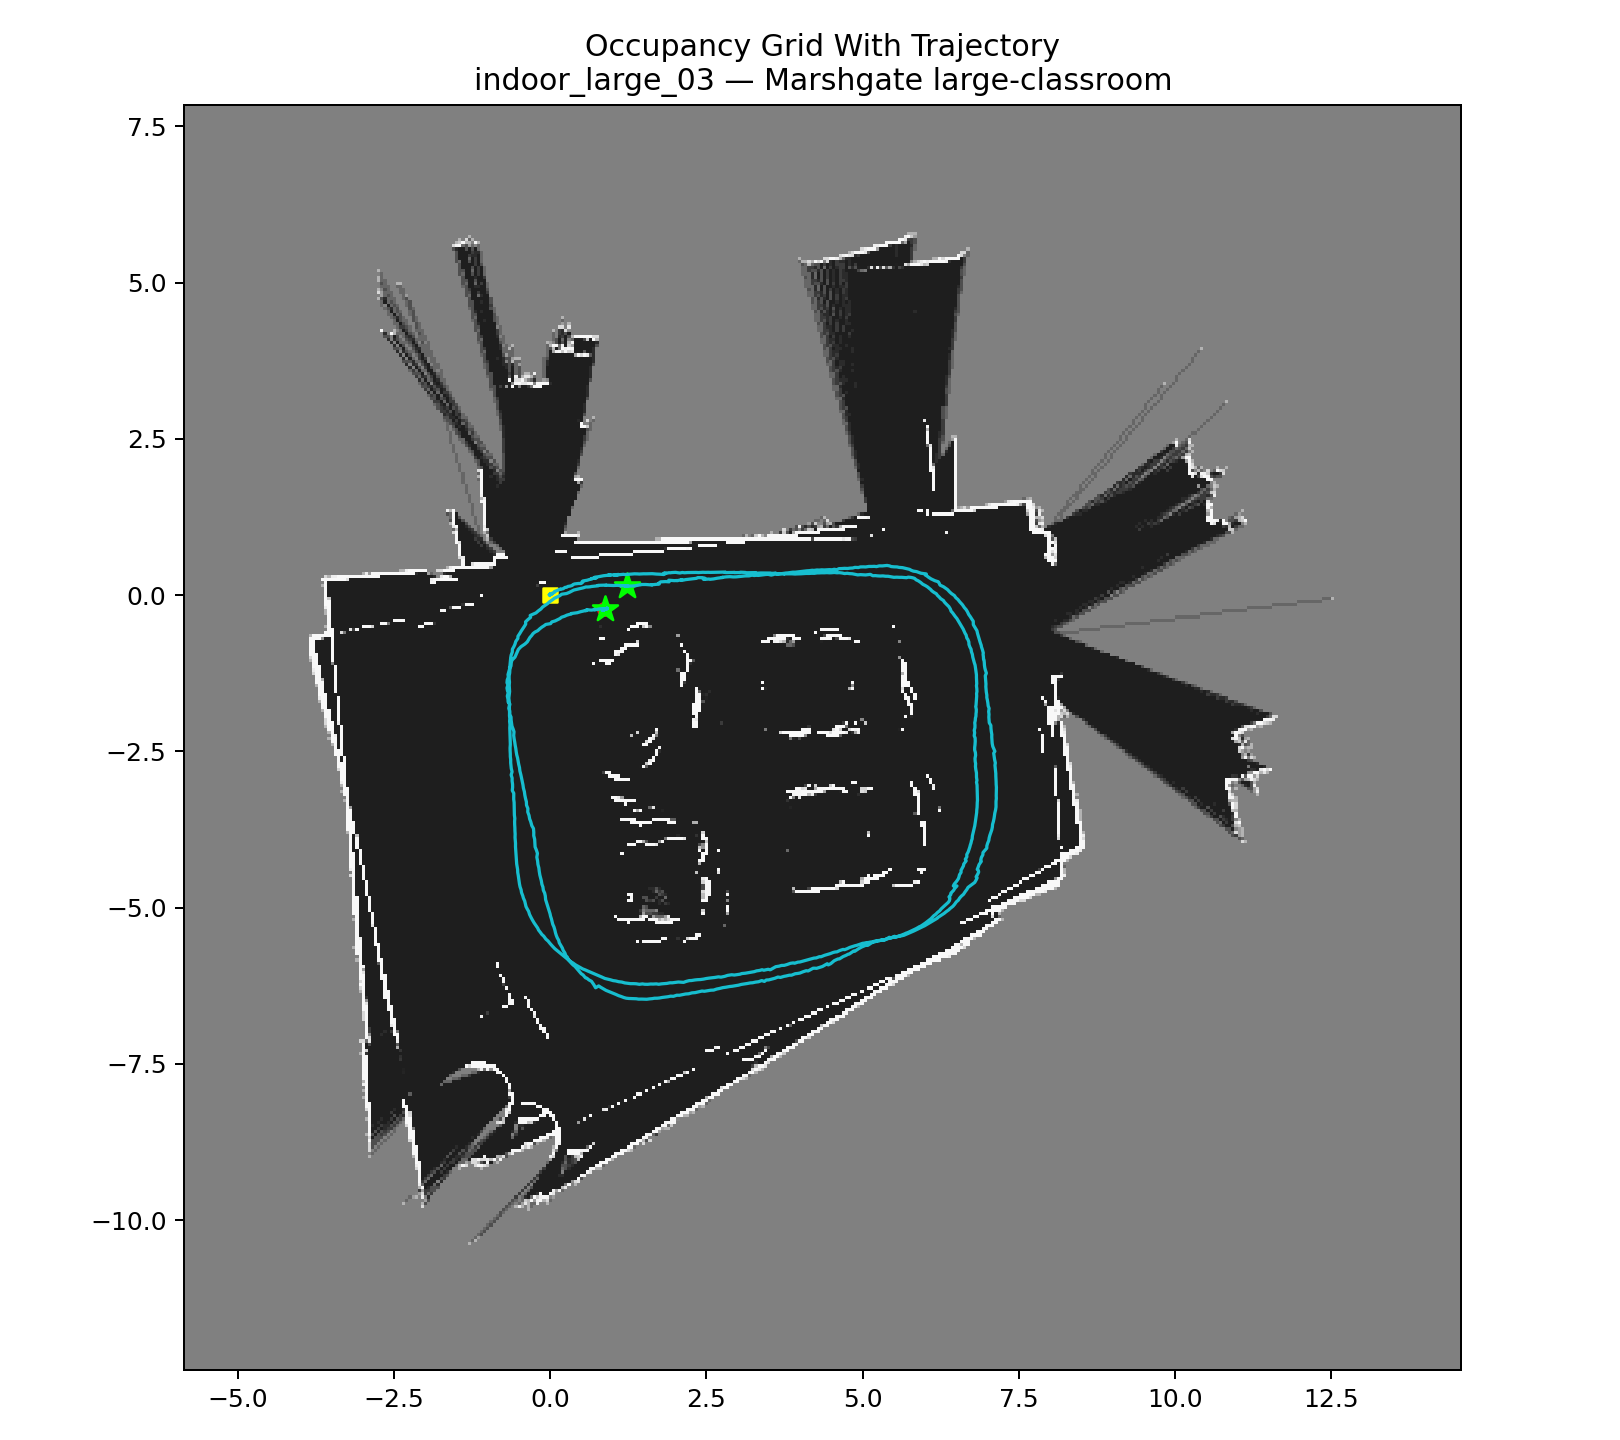
\includegraphics[width=\textwidth,height=0.43\textheight,keepaspectratio]{baseline_indoor_large.png}
          \par\vspace{0.2em}
          {\scriptsize Large classroom: stable walls and furniture returns.\par}
        \end{column}
        \begin{column}{0.49\textwidth}
          \centering
          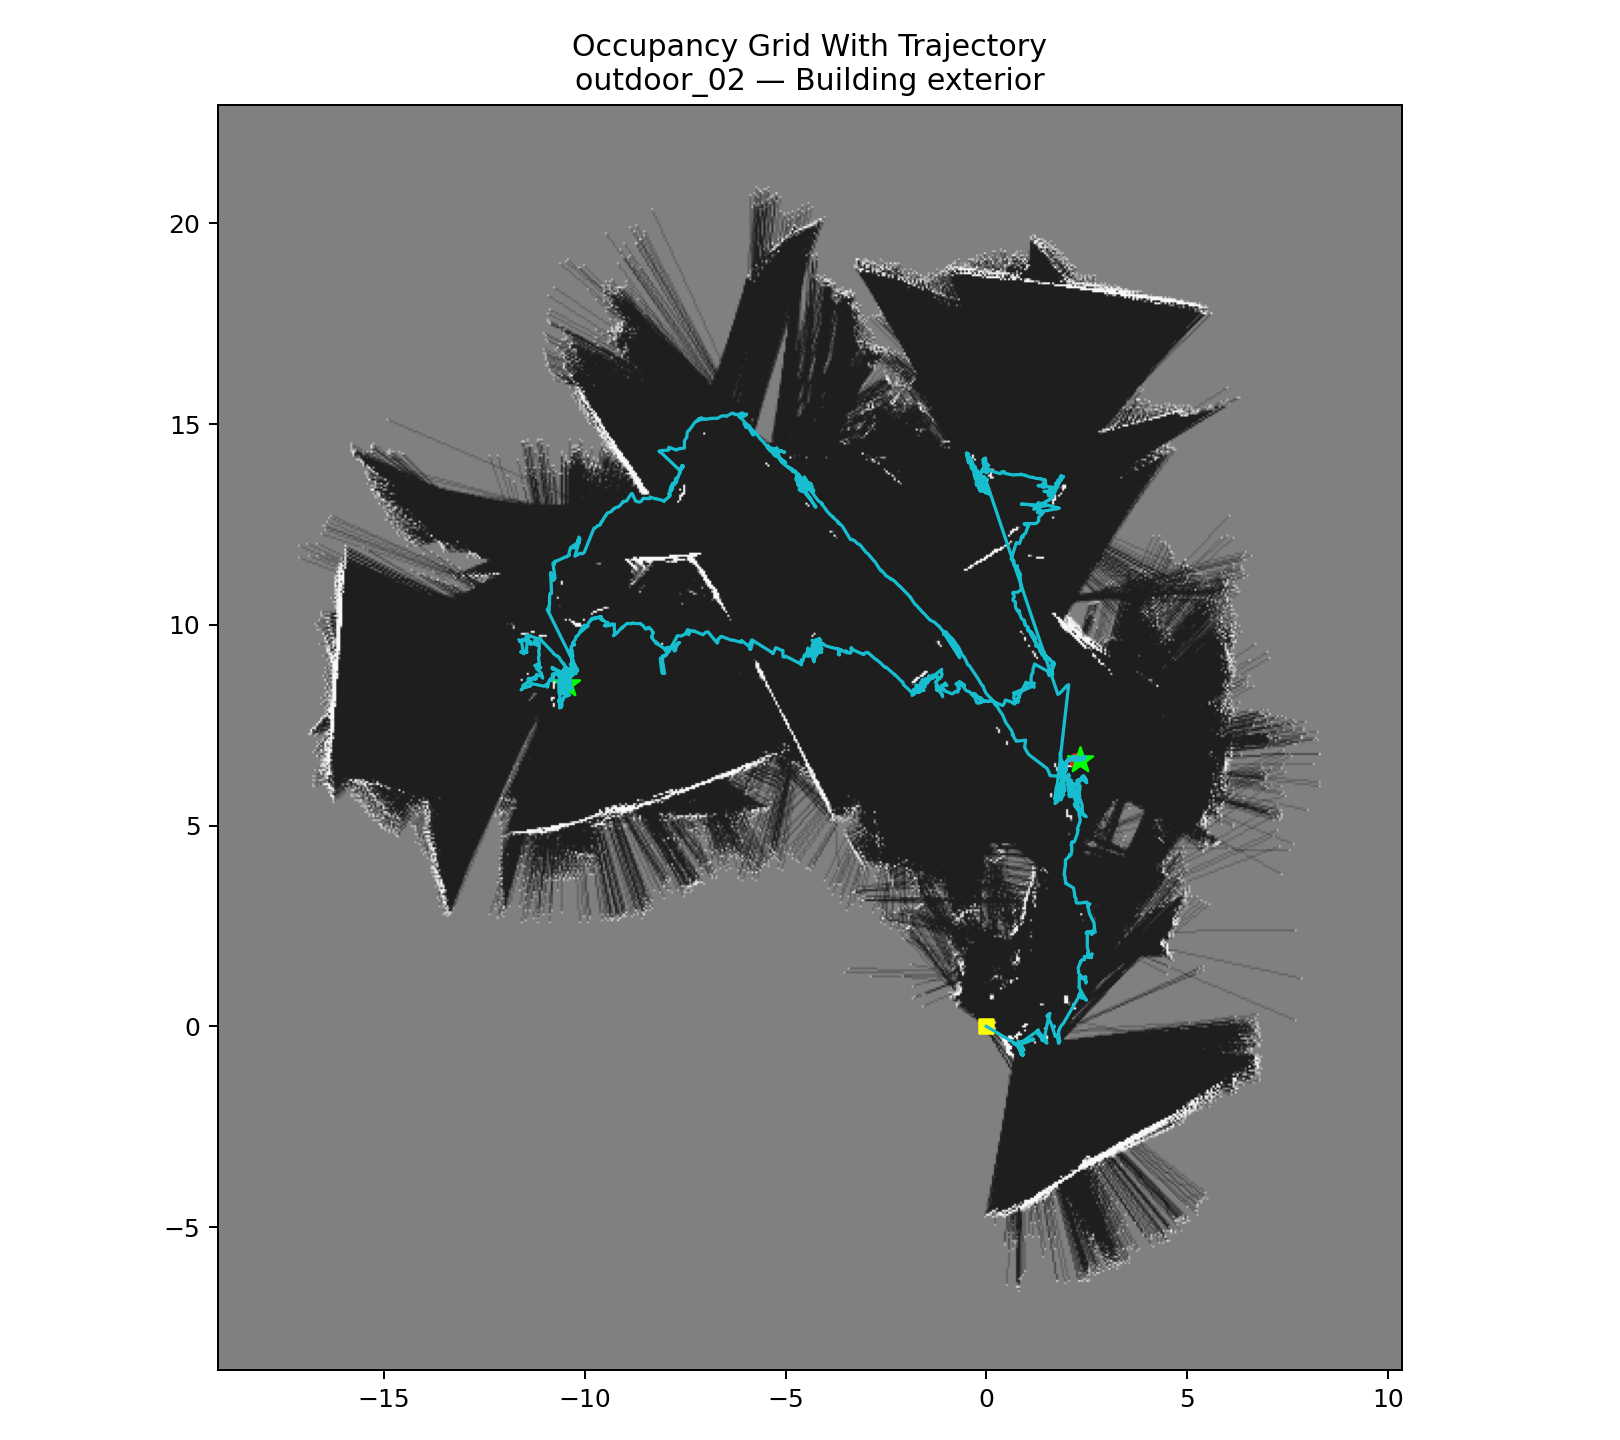
\includegraphics[width=\textwidth,height=0.43\textheight,keepaspectratio]{baseline_outdoor.png}
          \par\vspace{0.2em}
          {\scriptsize Outdoor: long route, visible drift.\par}
        \end{column}
      \end{columns}
    \end{column}
    \begin{column}{0.37\textwidth}
      \textbf{Baseline:} match each scan against the growing map, then build point-cloud and occupancy-grid maps.

      \vspace{0.5em}
      \centering
      \tiny
      \begin{tabular}{lccc}
      \toprule
      Case & Class. & Room & Outdoor \\
      \midrule
      Drift (m) & 0.886 & 3.586 & 7.000 \\
      \bottomrule
      \end{tabular}

      \vspace{0.7em}
      \raggedright
      \textbf{Parameter result:} no single setting is best everywhere. Useful scan detail depends on scene scale and structure.
    \end{column}
  \end{columns}
\end{frame}

\subsection{Loop Closure}

\begin{frame}{Loop-Closure Detection}
  \small
  \begin{columns}[T,onlytextwidth]
    \begin{column}{0.52\textwidth}
      \centering
      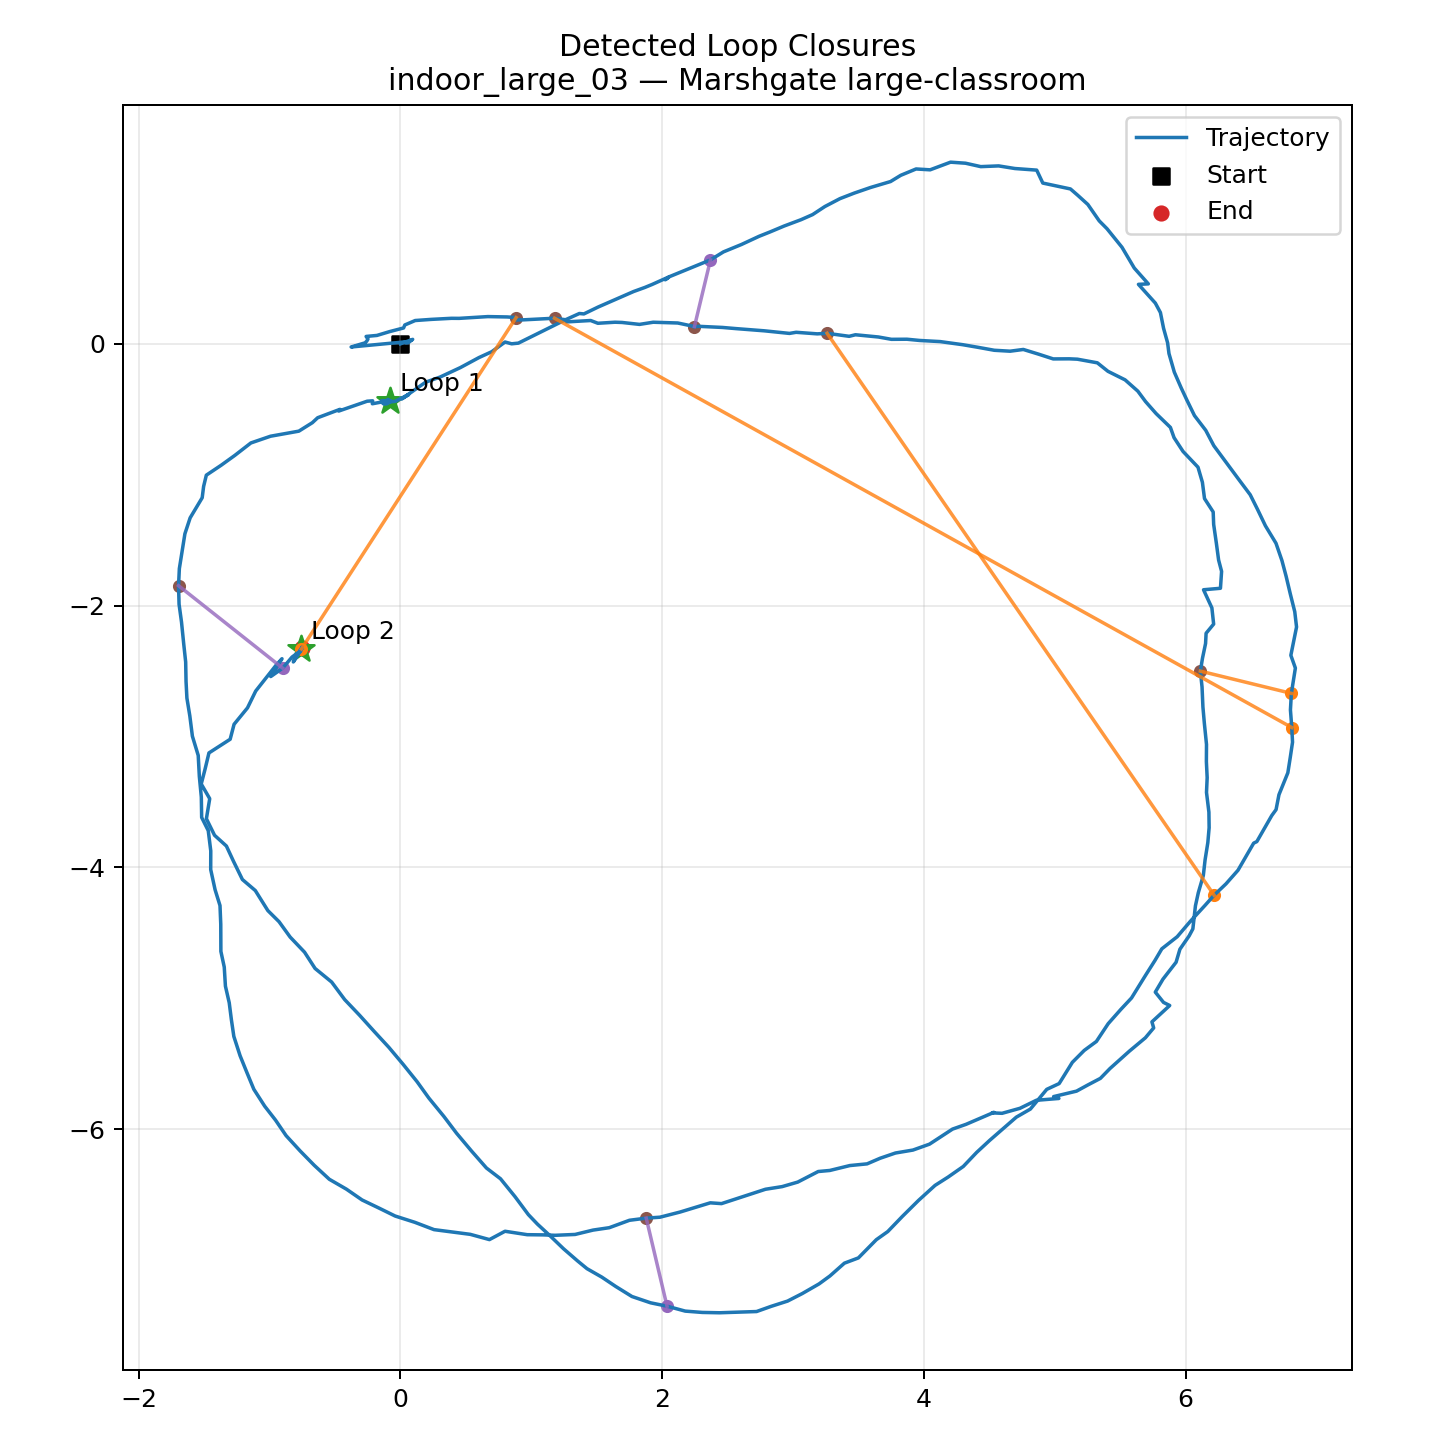
\includegraphics[width=\textwidth,height=0.56\textheight,keepaspectratio]{loop_indoor_large.png}
      \par\vspace{0.2em}
      {\scriptsize Large classroom loop detections.\par}
    \end{column}
    \begin{column}{0.44\textwidth}
      \textbf{Detection logic:} compare keyframes against earlier places, reject nearby-in-time candidates, verify alignment, then deduplicate repeated matches.

      \vspace{0.5em}
      \centering
      \scriptsize
      \begin{tabular}{lcc}
      \toprule
      Sequence & Loops & Marker hits \\
      \midrule
      Large classroom & 7 & 2/2 \\
      Small room & 4 & 1/2 \\
      Outdoor & 12 & 0/2 \\
      \bottomrule
      \end{tabular}

      \vspace{0.7em}
      \raggedright
      \scriptsize Outdoor marker hits are weak, but repeated places are still found.
    \end{column}
  \end{columns}
\end{frame}

\subsection{Optimisation}

\begin{frame}{Pose-Graph Optimisation}
  \small
  \begin{columns}[T,onlytextwidth]
    \begin{column}{0.58\textwidth}
      \centering
      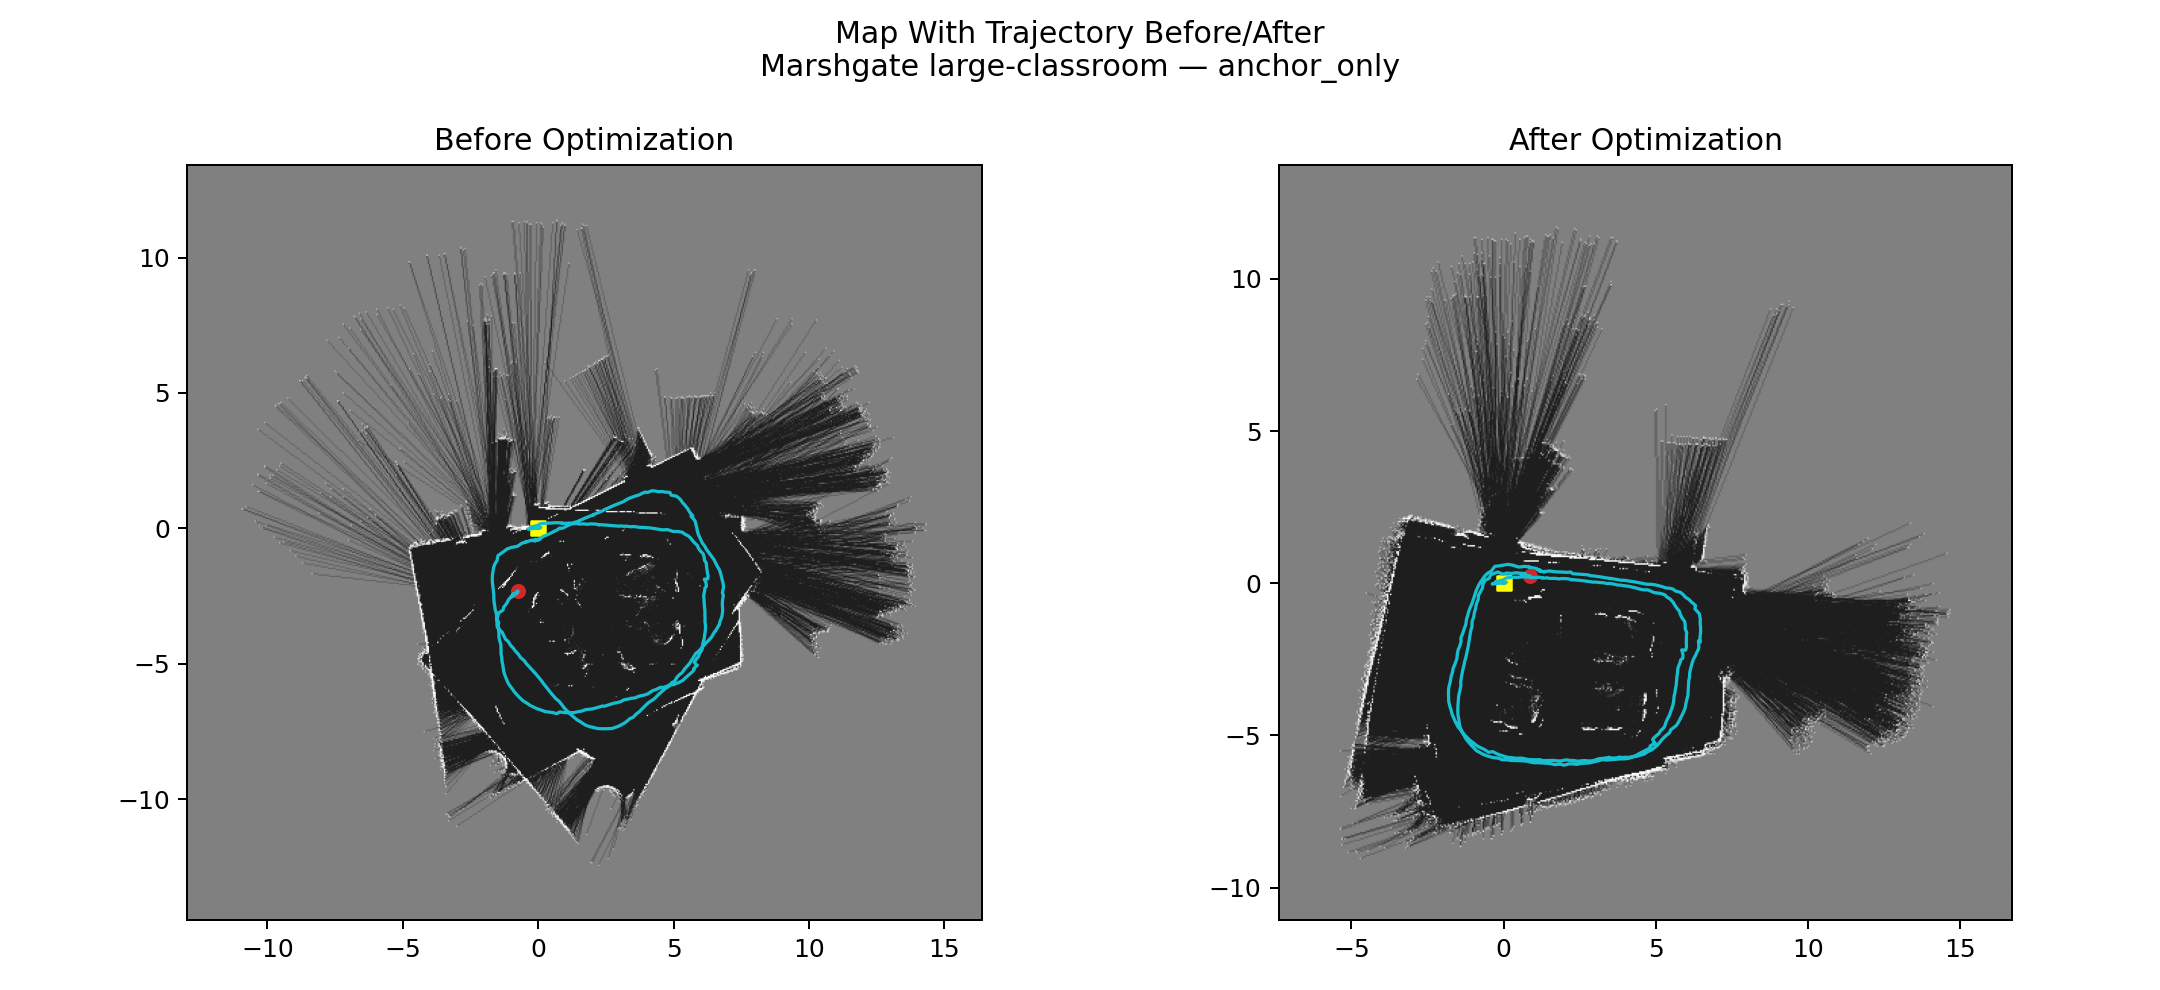
\includegraphics[width=\textwidth,height=0.29\textheight,keepaspectratio]{optim_indoor_large.png}
      \par\vspace{0.2em}
      {\scriptsize Large classroom: final pose moves closer to the start.\par}
      \vspace{0.5em}
      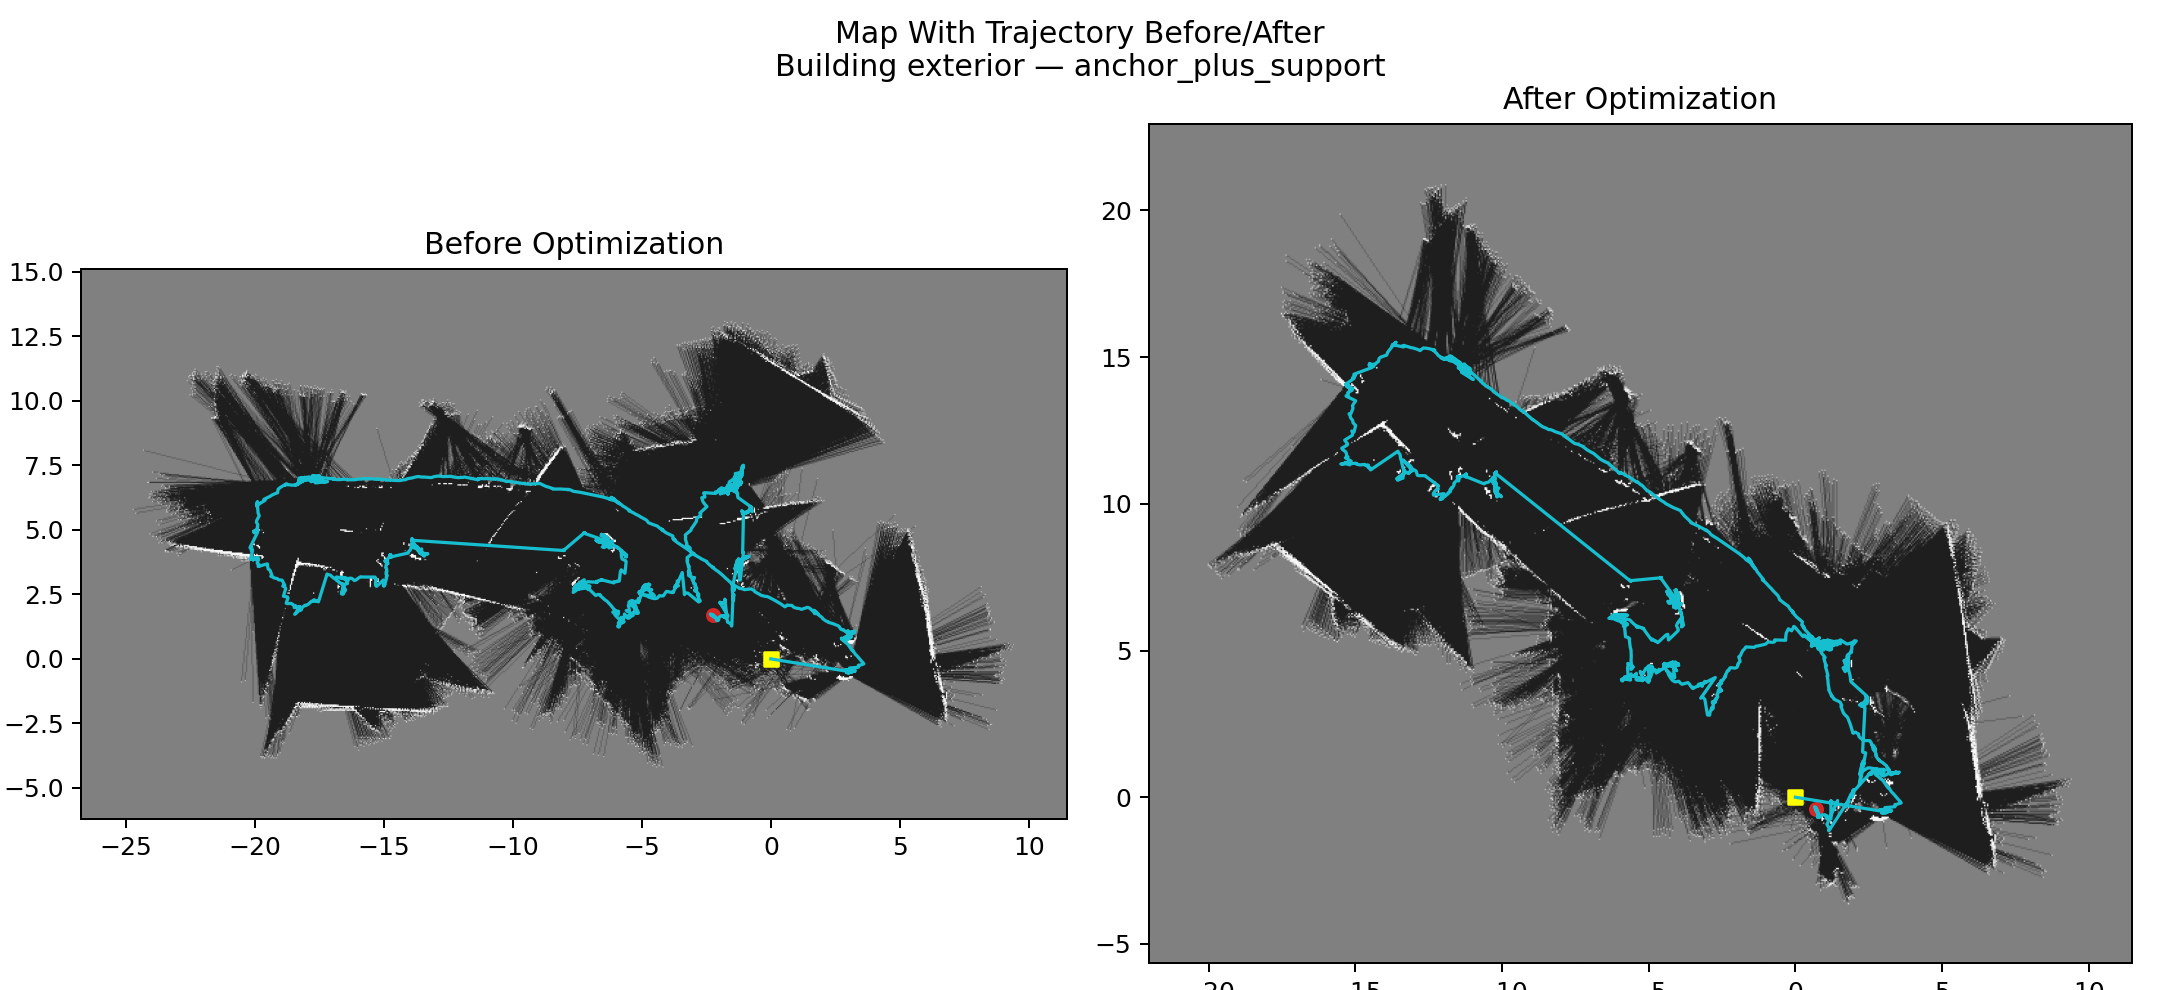
\includegraphics[width=\textwidth,height=0.29\textheight,keepaspectratio]{optim_outdoor.png}
      \par\vspace{0.2em}
      {\scriptsize Outdoor: two loop edges close the route more smoothly.\par}
    \end{column}
    \begin{column}{0.38\textwidth}
      \begin{block}{What changed}
        Odometry links keep the local path shape, and loop links pull revisited places back together.
      \end{block}
      \vspace{0.3em}
      \begin{table}
      \centering
      \scriptsize
      \begin{tabular}{lcc}
      \toprule
      Sequence & Before & After \\
      \midrule
      Large classroom & 2.443 & 0.898 \\
      Small room & 2.395 & 0.546 \\
      Outdoor & 2.820 & 0.817 \\
      \bottomrule
      \end{tabular}
      \end{table}
      \scriptsize Closure error in metres. Lower is better.
    \end{column}
  \end{columns}
\end{frame}

\begin{frame}{LiDAR Conclusion}
  \small
  \begin{columns}[T,onlytextwidth]
    \begin{column}{0.48\textwidth}
      \begin{block}{Main result}
        Laser odometry can build useful maps, but loop closure is needed to make the second loop consistent.
      \end{block}
      \vspace{0.2em}
      \begin{itemize}
        \item Parameter choices changed by environment.
        \item Loop detection found useful revisits in all three sequences.
        \item Optimisation reduced closure error for every sequence.
      \end{itemize}
    \end{column}
    \begin{column}{0.48\textwidth}
      \begin{table}
      \centering
      \scriptsize
      \begin{tabular}{lcc}
      \toprule
      Sequence & Loop edges & Improvement \\
      \midrule
      Large classroom & 1 & 1.546 m \\
      Small room & 1 & 1.848 m \\
      Outdoor & 2 & 2.003 m \\
      \bottomrule
      \end{tabular}
      \end{table}
      \vspace{0.1em}
      \scriptsize The outdoor result needs one supporting loop edge to close the route without bending it too much.
    \end{column}
  \end{columns}
\end{frame}

\begin{frame}{Thank You}
  \centering
  \vspace{1.5em}
  {\Huge Thank you}

  \vspace{1.2em}
  {\Large Questions?}

  \vspace{1.6em}
  {\small Group 6: David Zhong, Harry Tan, Yukun Wang}
\end{frame}

\appendix
\section{Backup}
\subsection{Q\&A}

\begin{frame}{Backup: Parameter Study Details}
  \centering
  \scriptsize
  \setlength{\tabcolsep}{4pt}
  \begin{tabular}{llccc}
  \toprule
  Study & Setting & Classroom & Room & Outdoor \\
  \midrule
  Range & 6 m & 0.886 & 3.586 & 7.000 \\
  Range & 12 m & 0.494 & 2.301 & 18.183 \\
  Beams & Full & 0.886 & 3.586 & 7.000 \\
  Beams & 1/2 & 0.451 & 4.782 & 9.203 \\
  Beams & 1/3 & 0.852 & 2.258 & 7.875 \\
  Voxel & 0.05 m & 0.886 & 3.586 & 7.000 \\
  Voxel & 0.10 m & 0.886 & 3.674 & 2251.157 \\
  Scans & All & 0.886 & 3.586 & 7.000 \\
  Scans & 1/2 & 0.915 & 0.608 & 2.820 \\
  Scans & 1/3 & 0.687 & 1.978 & 3.708 \\
  \bottomrule
  \end{tabular}

  \vspace{0.6em}
  \smallcaption{Final drift in metres. The 0.10 m voxel outdoor case failed badly because too much local structure was removed.}
\end{frame}

\begin{frame}{Backup: Parameter Figures}
  \begin{columns}[T,onlytextwidth]
    \begin{column}{0.49\textwidth}
      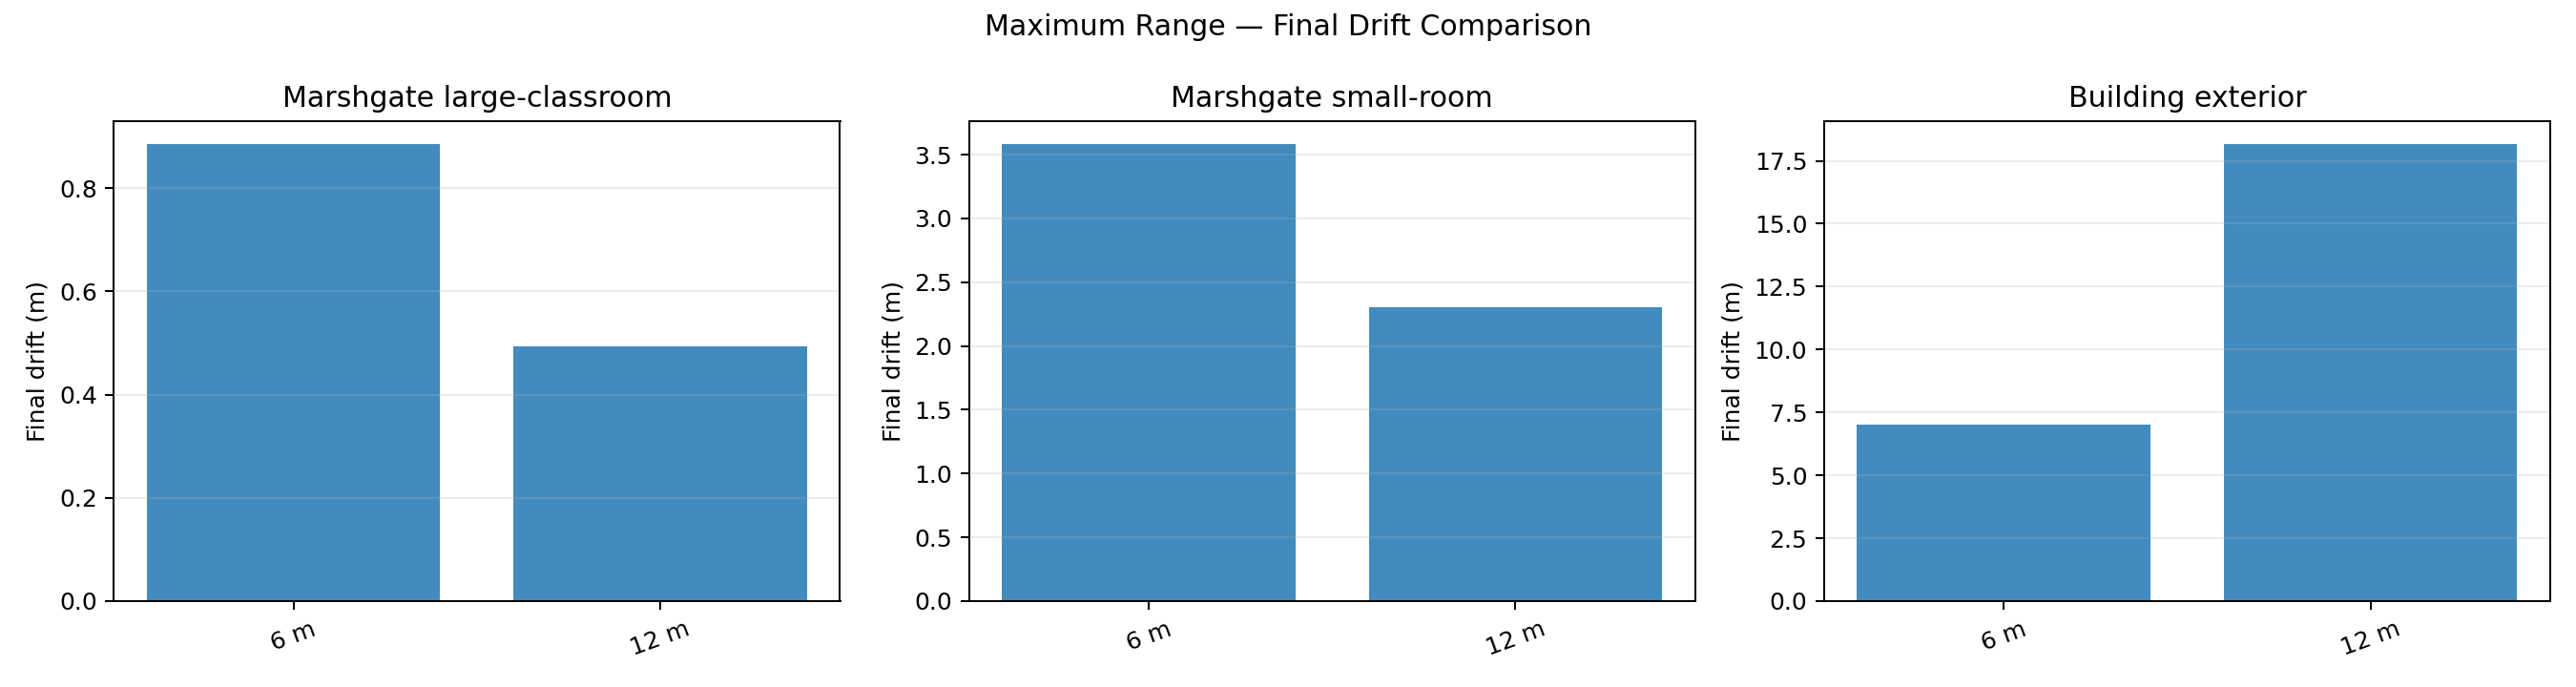
\includegraphics[width=\textwidth]{param_max_range.png}
      \vspace{0.3em}
      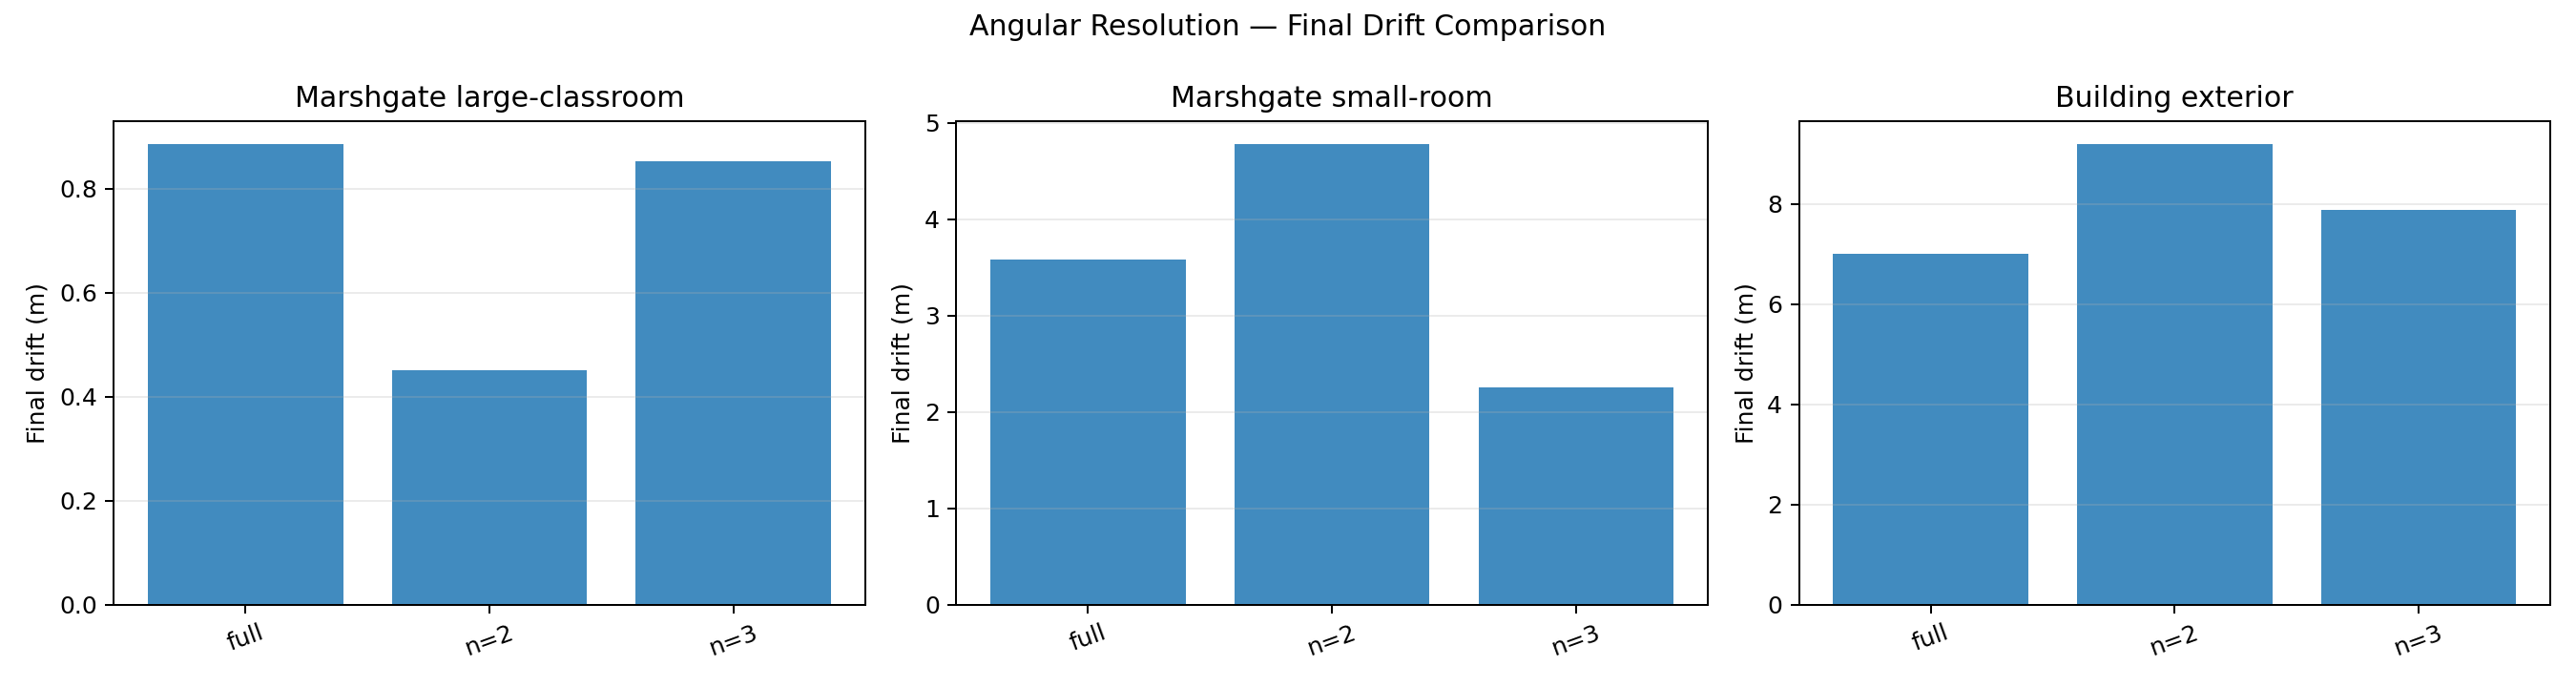
\includegraphics[width=\textwidth]{param_angular_resolution.png}
    \end{column}
    \begin{column}{0.49\textwidth}
      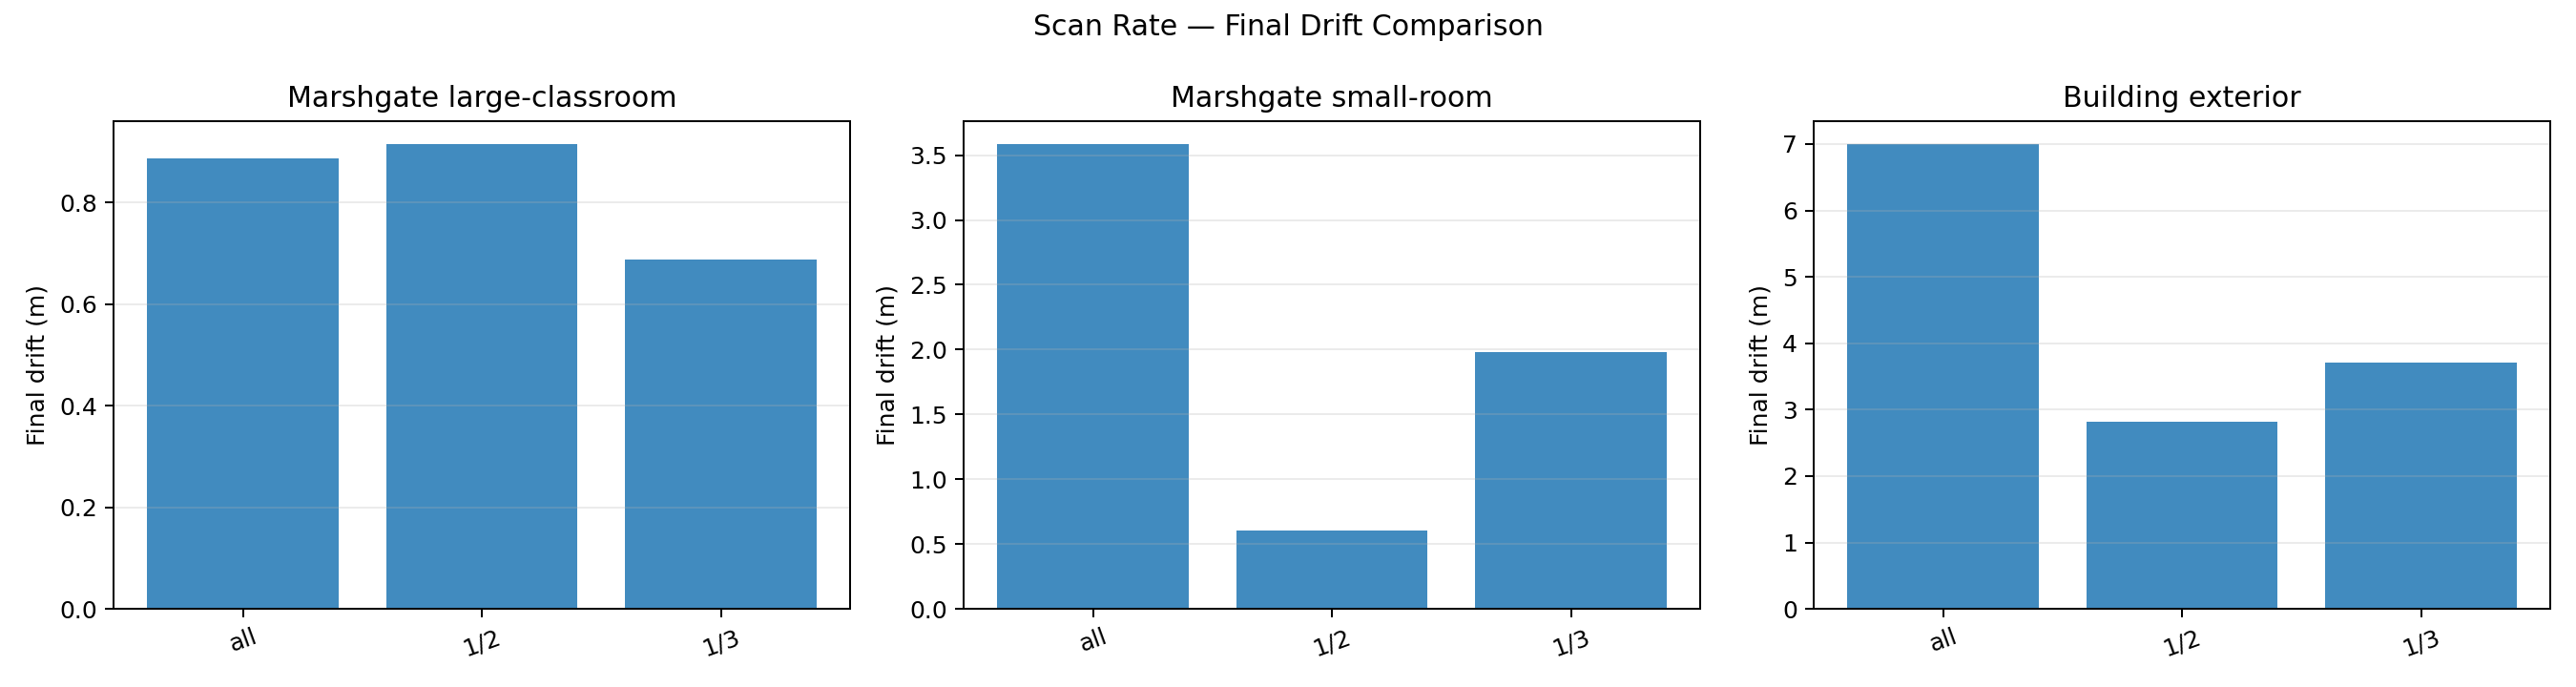
\includegraphics[width=\textwidth]{param_scan_rate.png}
      \vspace{0.3em}
      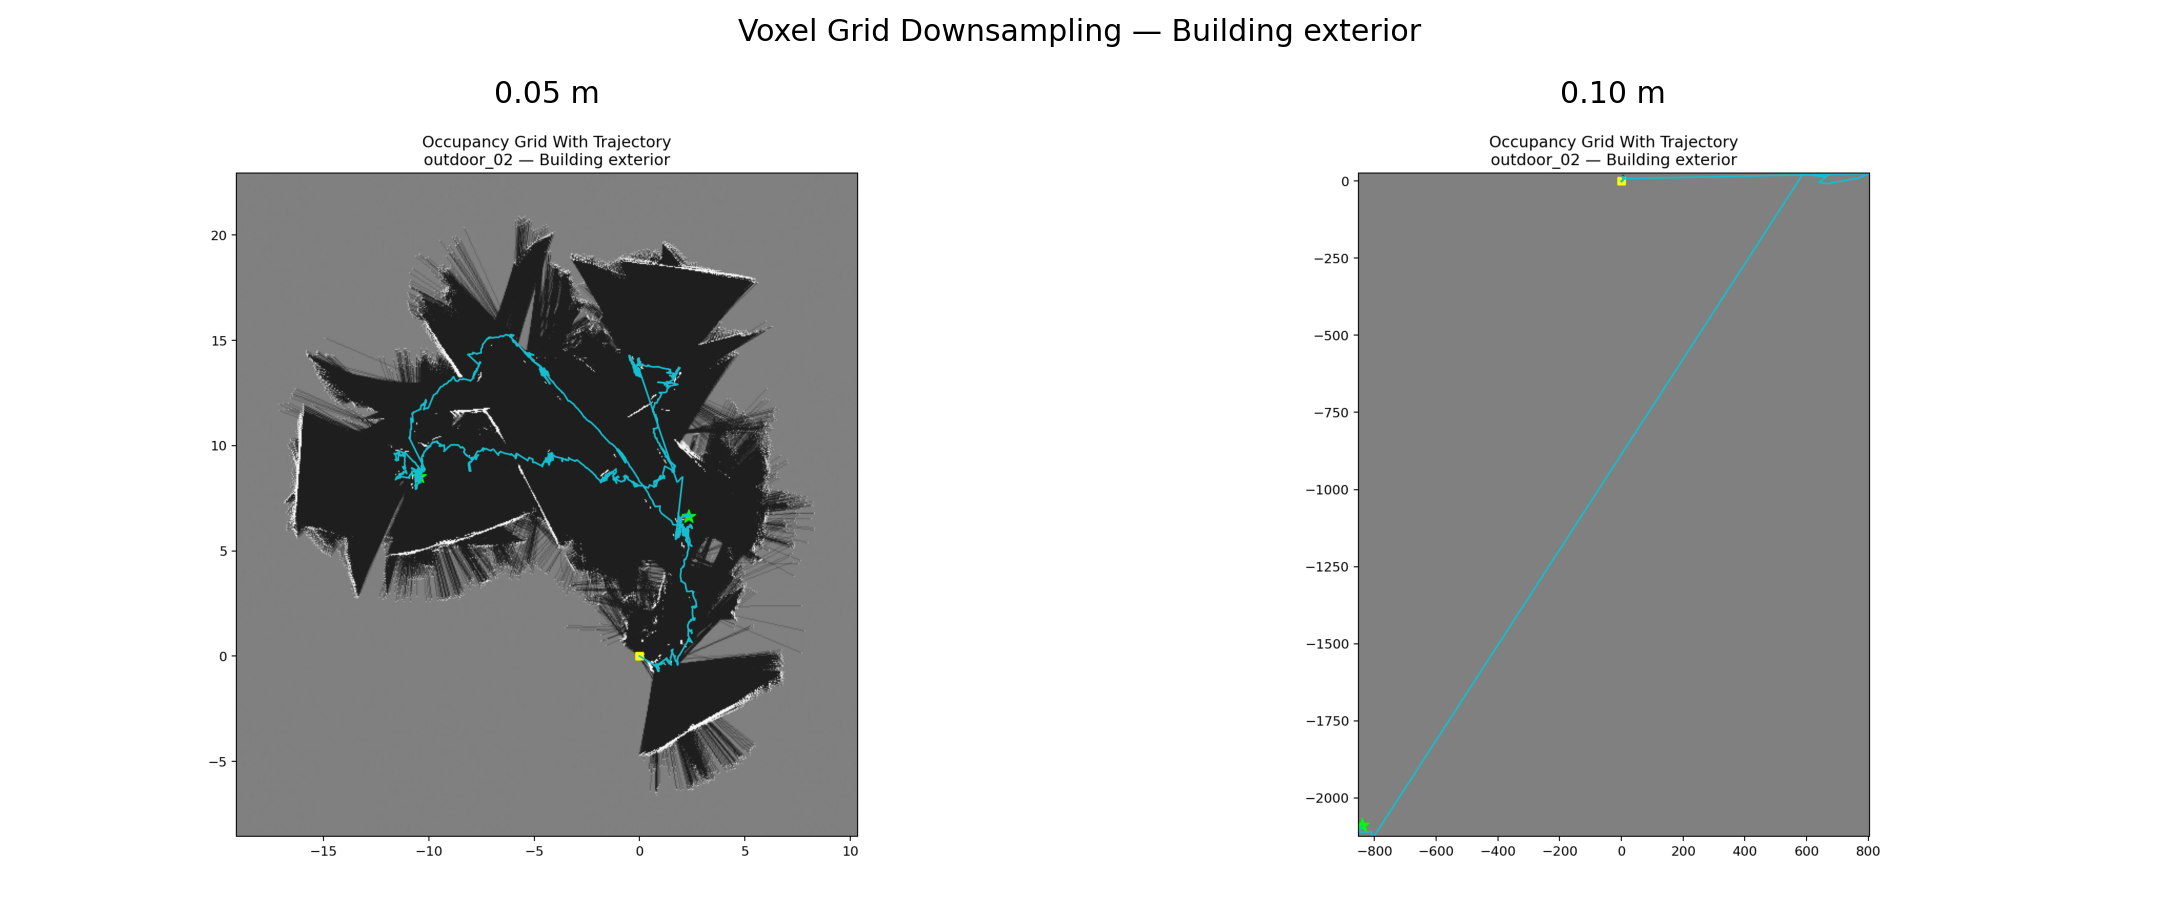
\includegraphics[width=\textwidth]{param_voxel_outdoor.png}
    \end{column}
  \end{columns}
\end{frame}

\begin{frame}{Backup: Loop Detections by Sequence}
  \begin{columns}[T,onlytextwidth]
    \begin{column}{0.32\textwidth}
      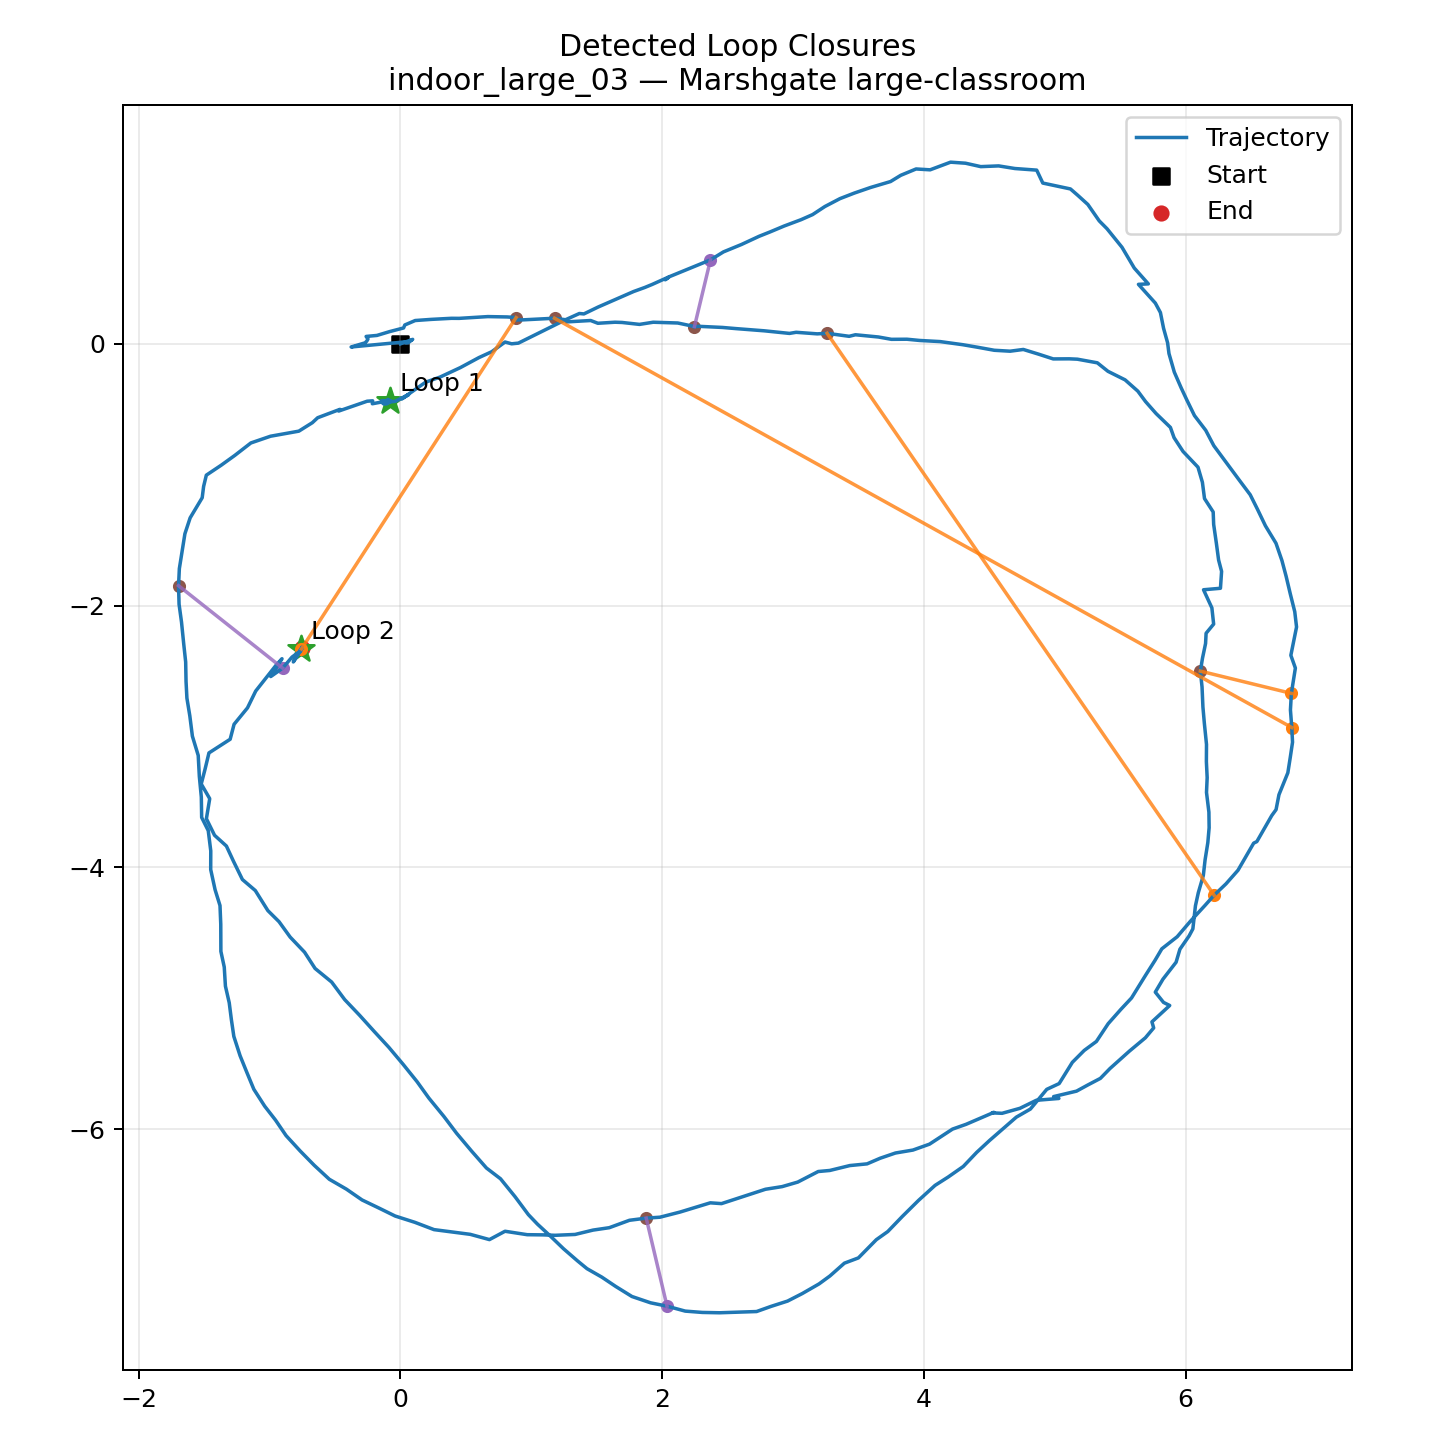
\includegraphics[width=\textwidth]{loop_indoor_large.png}
      \centering\scriptsize Large classroom: 7 loops, 2/2 marker hits
    \end{column}
    \begin{column}{0.32\textwidth}
      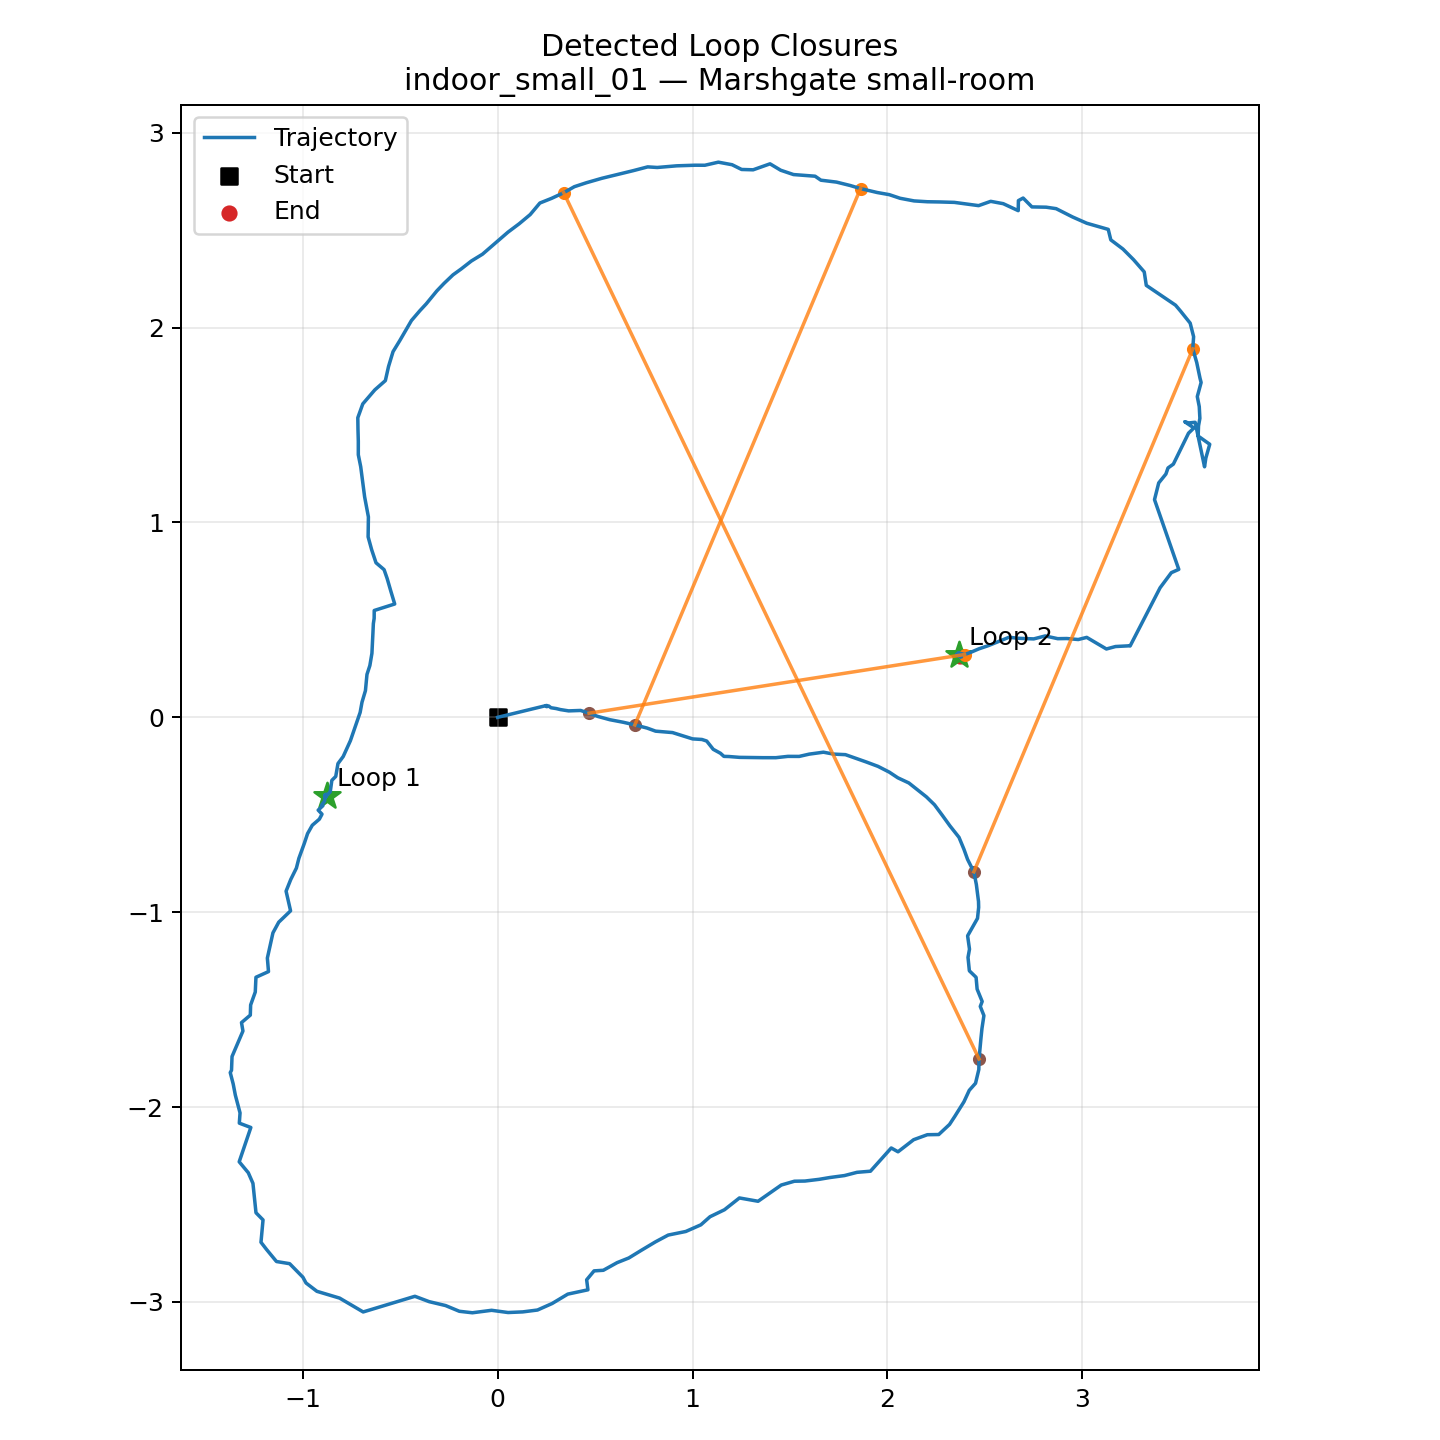
\includegraphics[width=\textwidth]{loop_indoor_small.png}
      \centering\scriptsize Small room: 4 loops, 1/2 marker hits
    \end{column}
    \begin{column}{0.32\textwidth}
      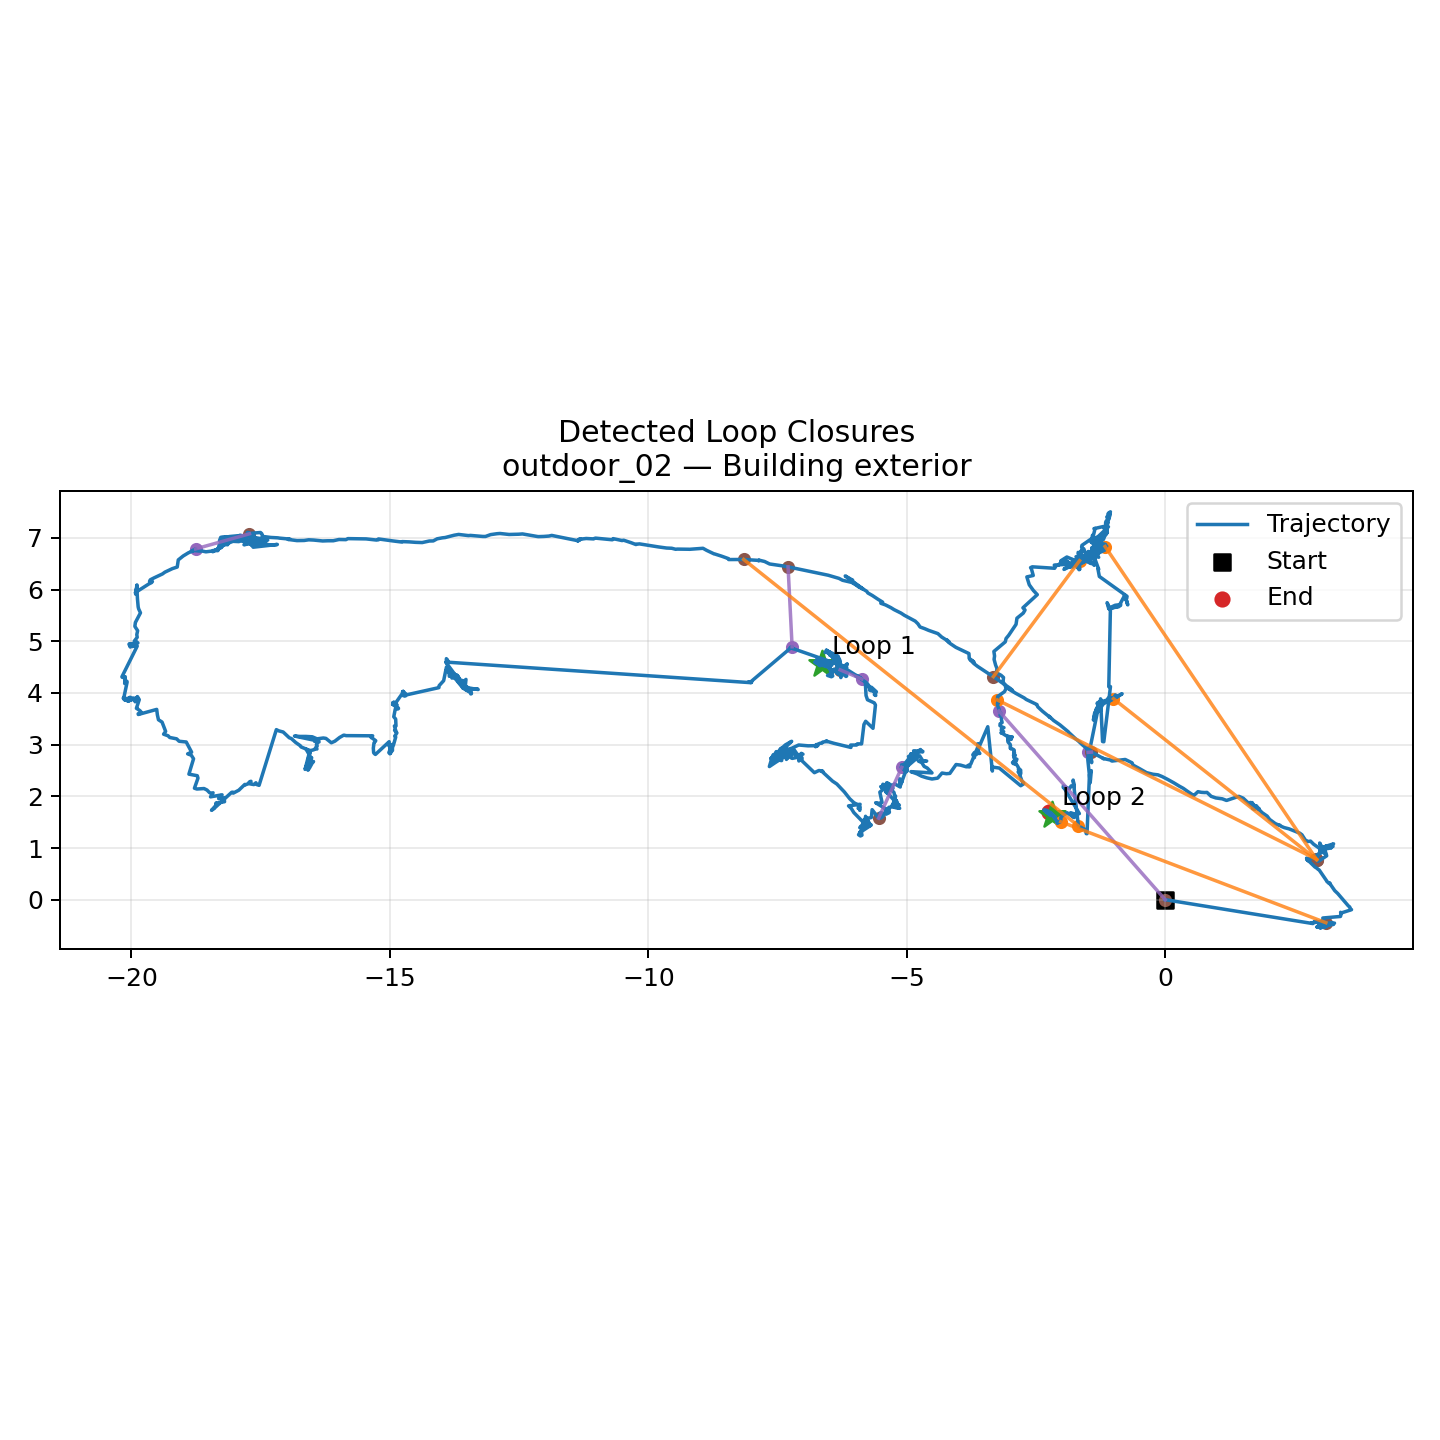
\includegraphics[width=\textwidth]{loop_outdoor.png}
      \centering\scriptsize Outdoor: 12 loops, 0/2 marker hits
    \end{column}
  \end{columns}
\end{frame}

\begin{frame}{Backup: Optimisation by Sequence}
  \begin{columns}[T,onlytextwidth]
    \begin{column}{0.33\textwidth}
      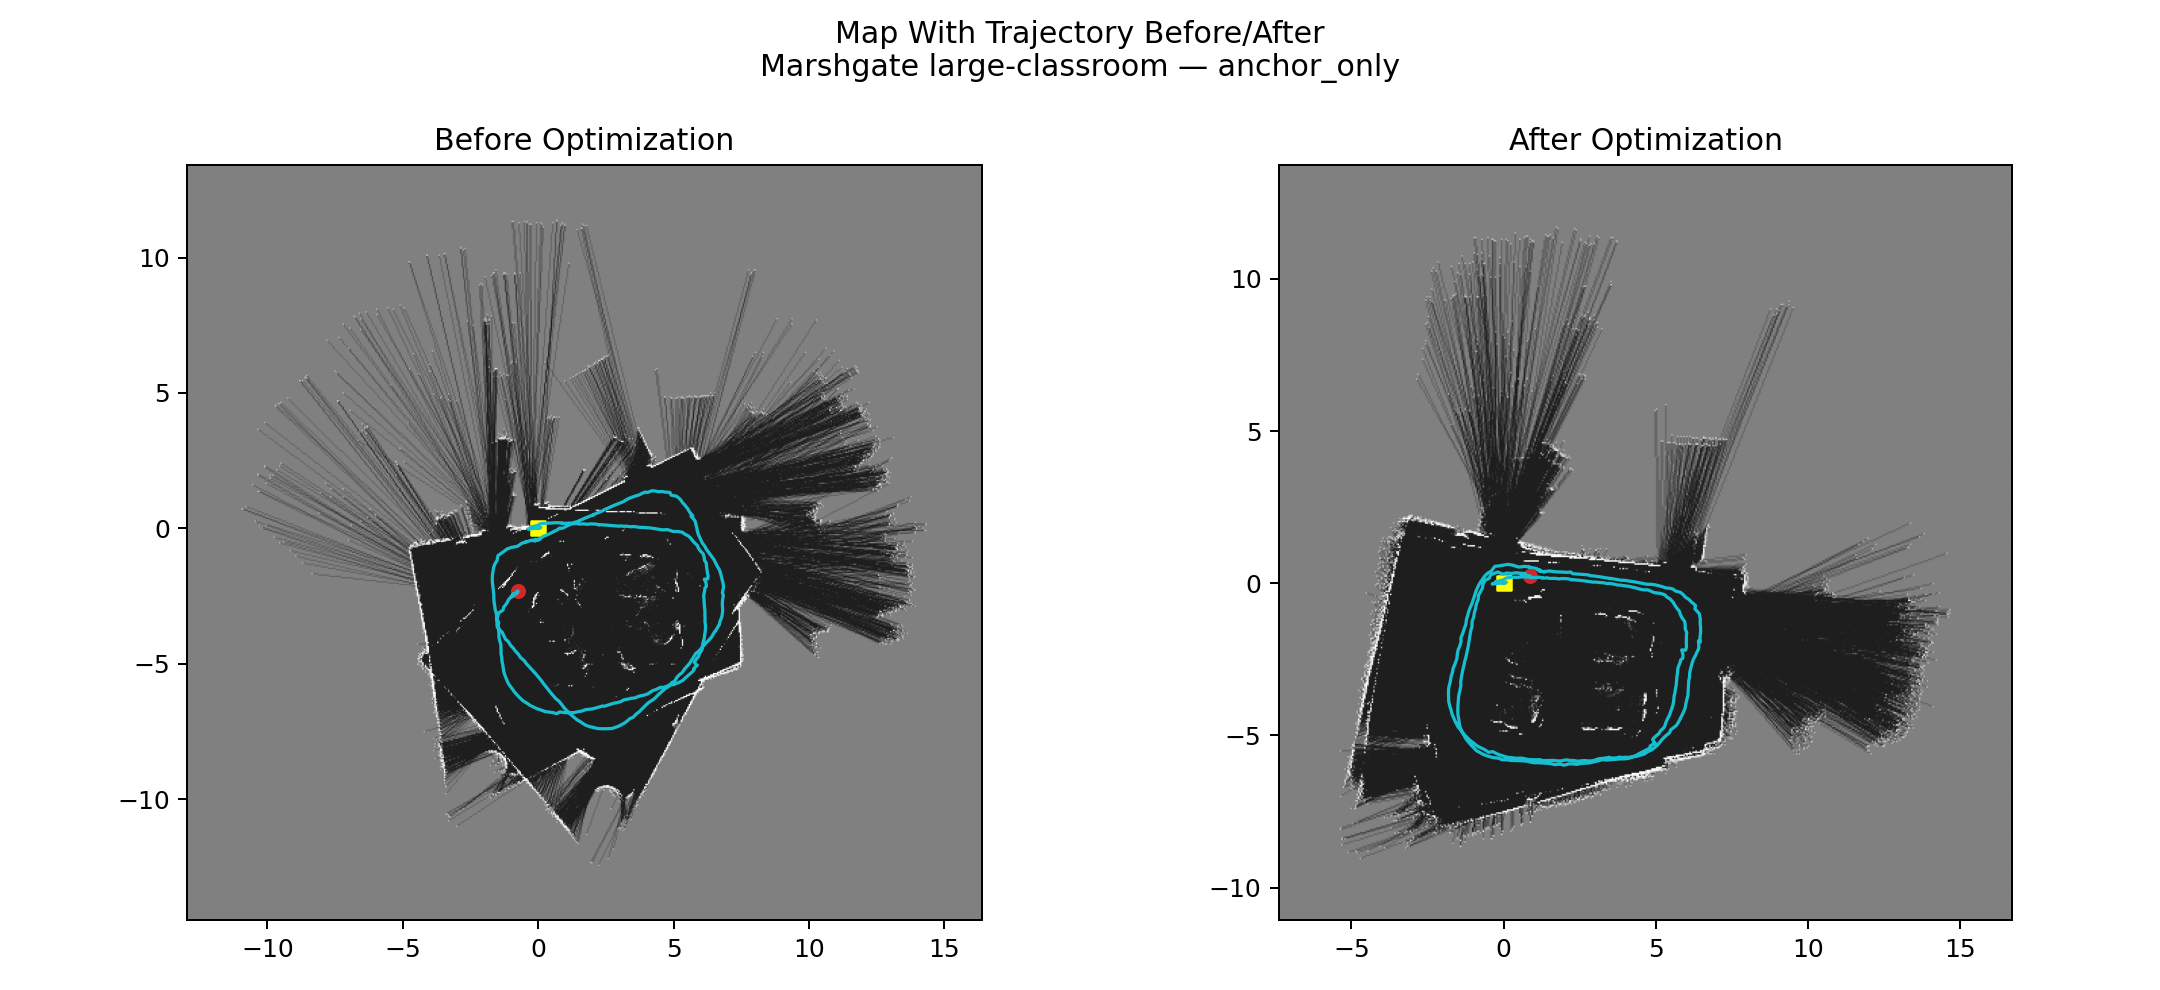
\includegraphics[width=\textwidth]{optim_indoor_large.png}
      \centering\scriptsize Large classroom: 2.443 m to 0.898 m
    \end{column}
    \begin{column}{0.33\textwidth}
      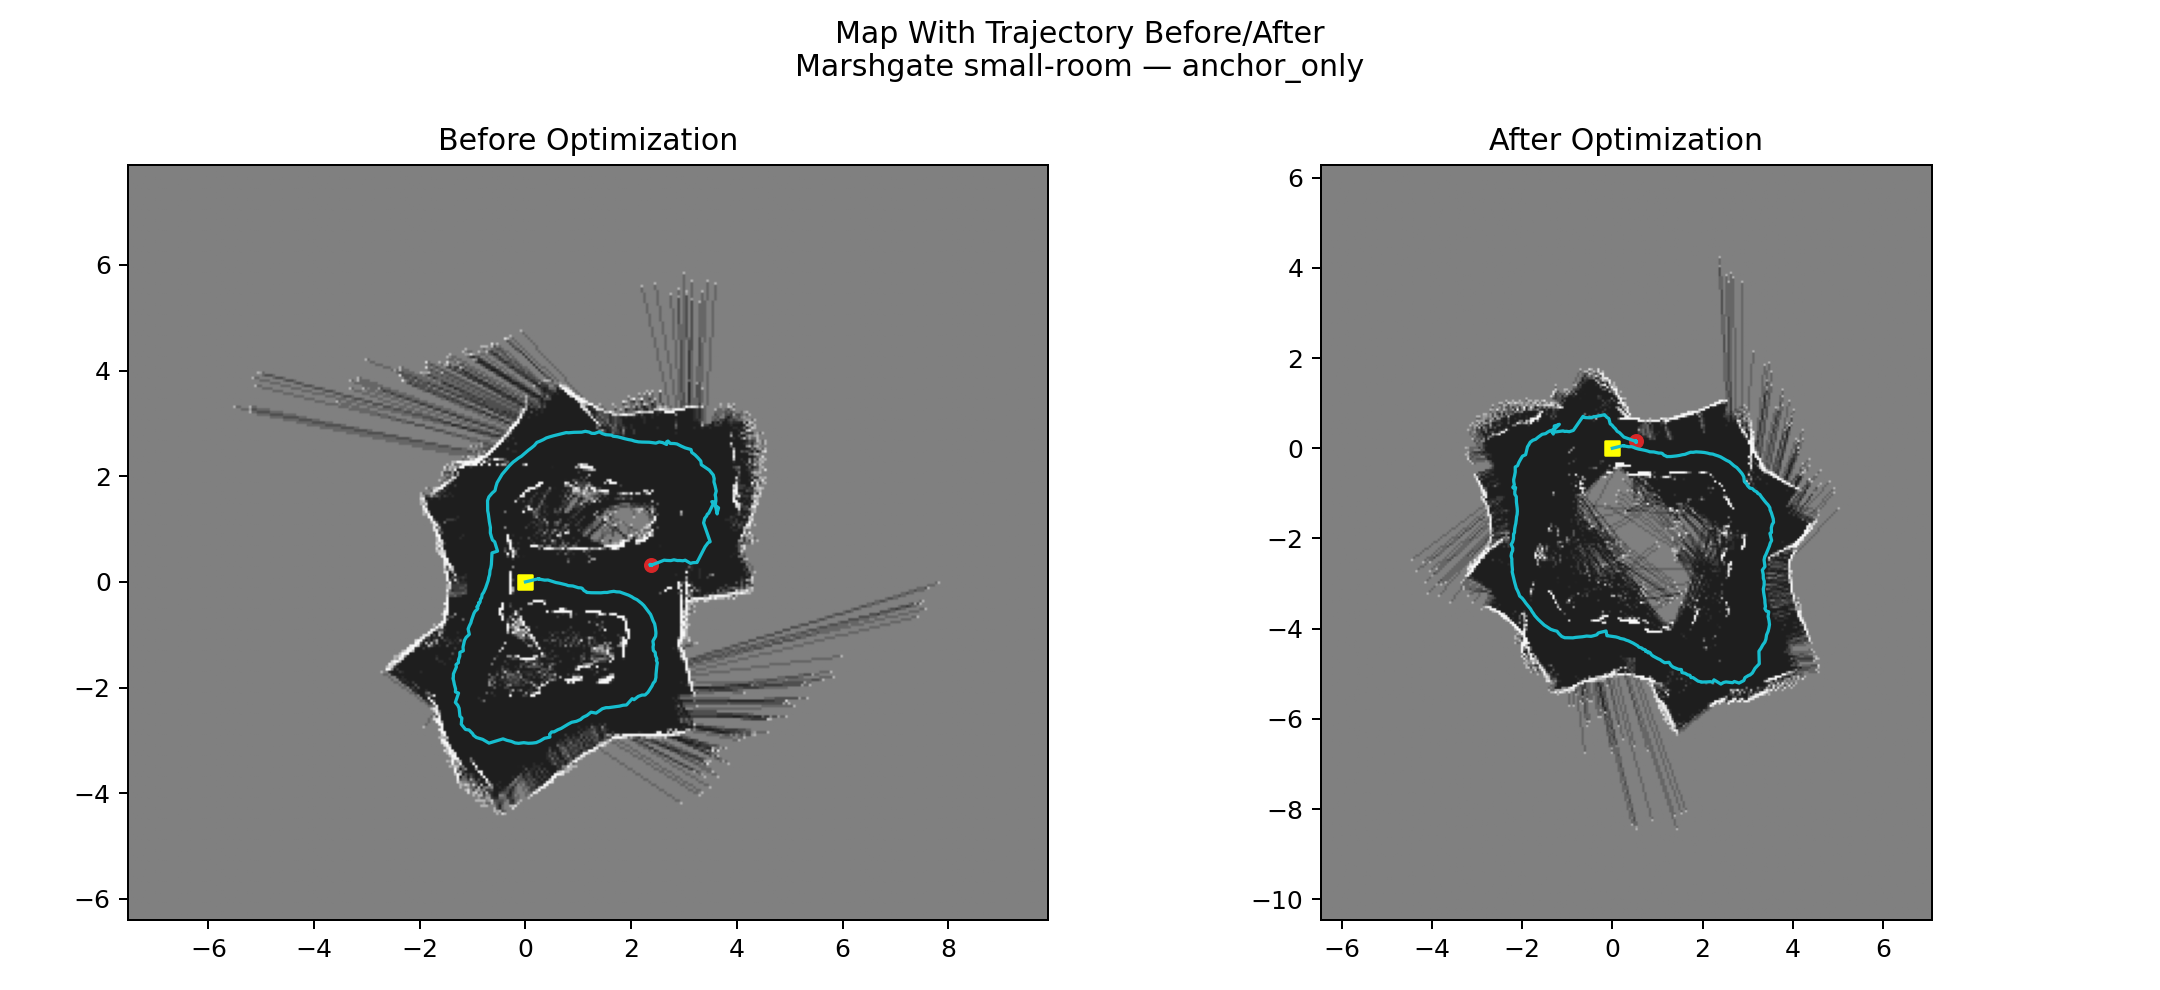
\includegraphics[width=\textwidth]{optim_indoor_small.png}
      \centering\scriptsize Small room: 2.395 m to 0.546 m
    \end{column}
    \begin{column}{0.33\textwidth}
      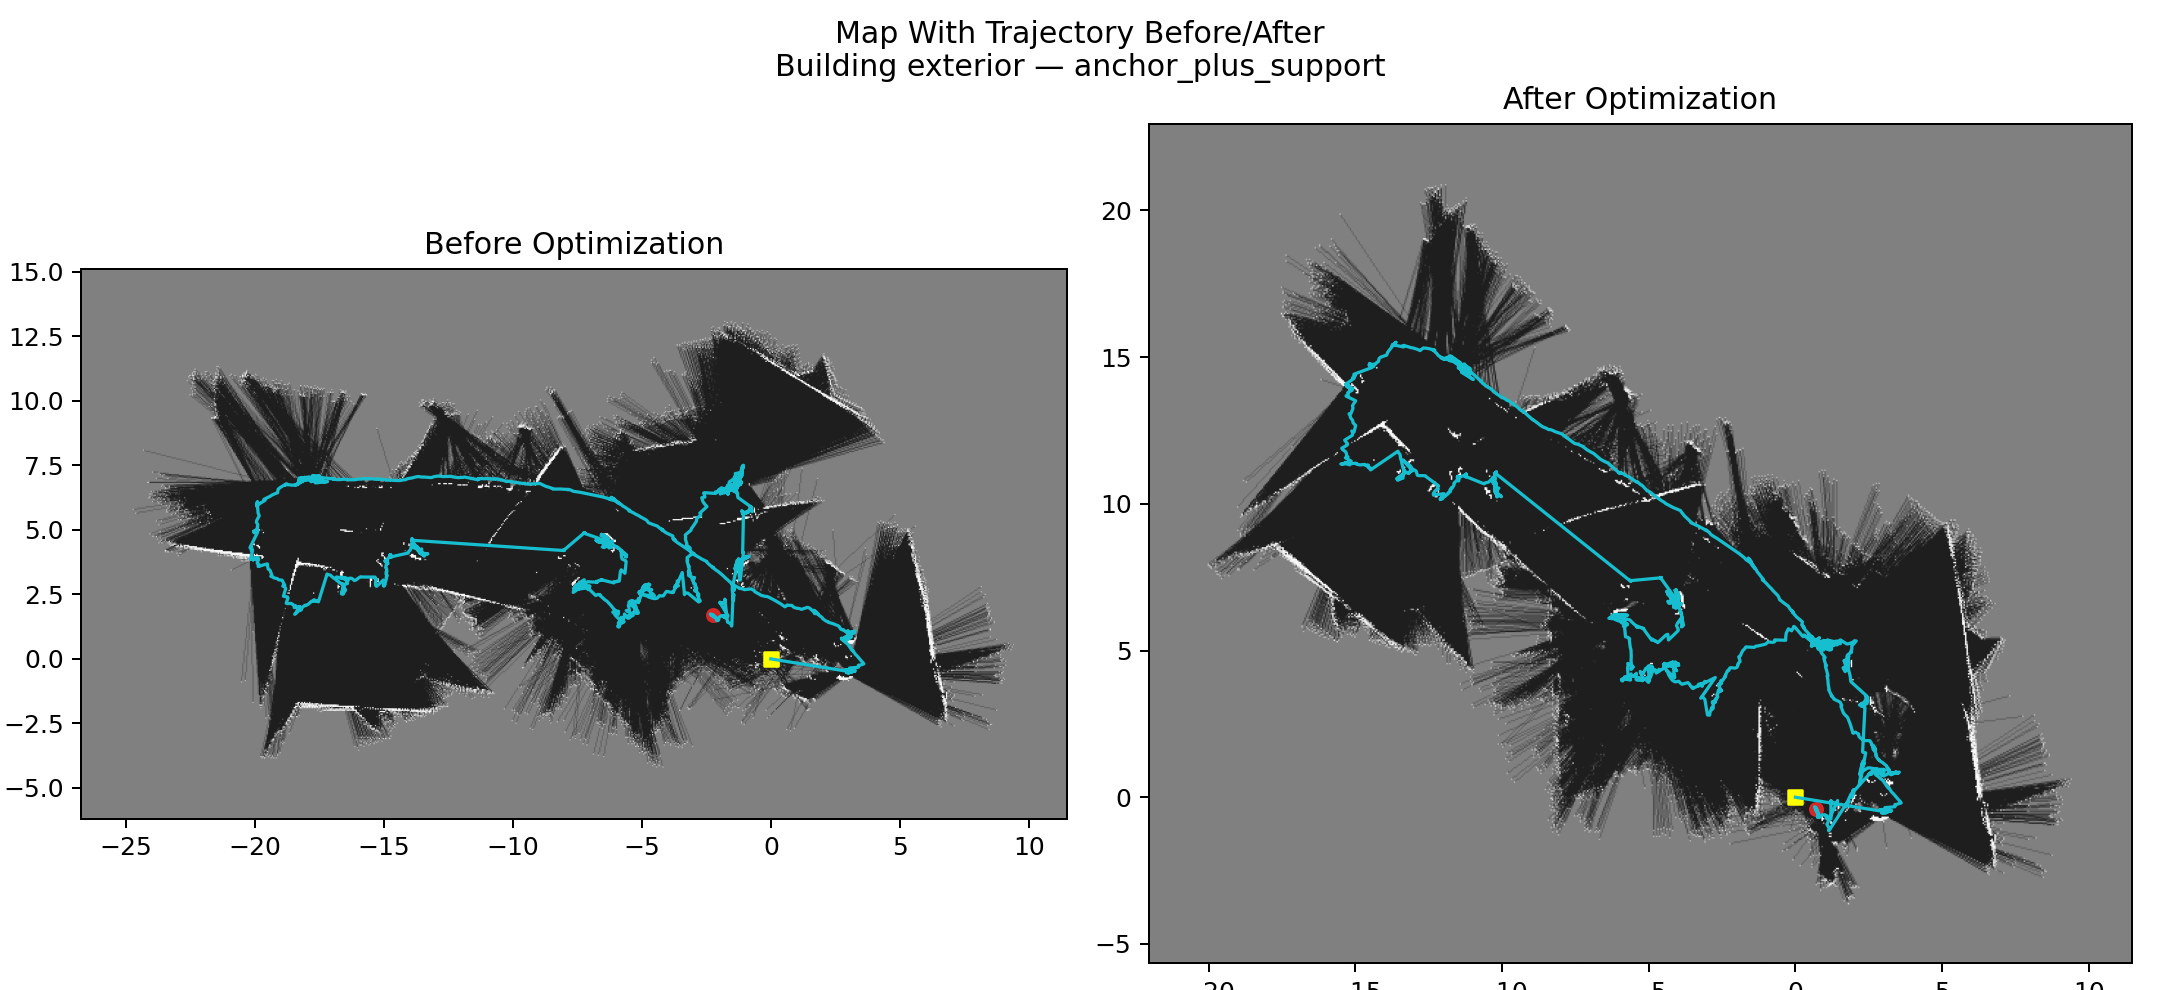
\includegraphics[width=\textwidth]{optim_outdoor.png}
      \centering\scriptsize Outdoor: 2.820 m to 0.817 m
    \end{column}
  \end{columns}
\end{frame}

\begin{frame}{Backup: Baseline Maps by Sequence}
  \begin{columns}[T,onlytextwidth]
    \begin{column}{0.32\textwidth}
      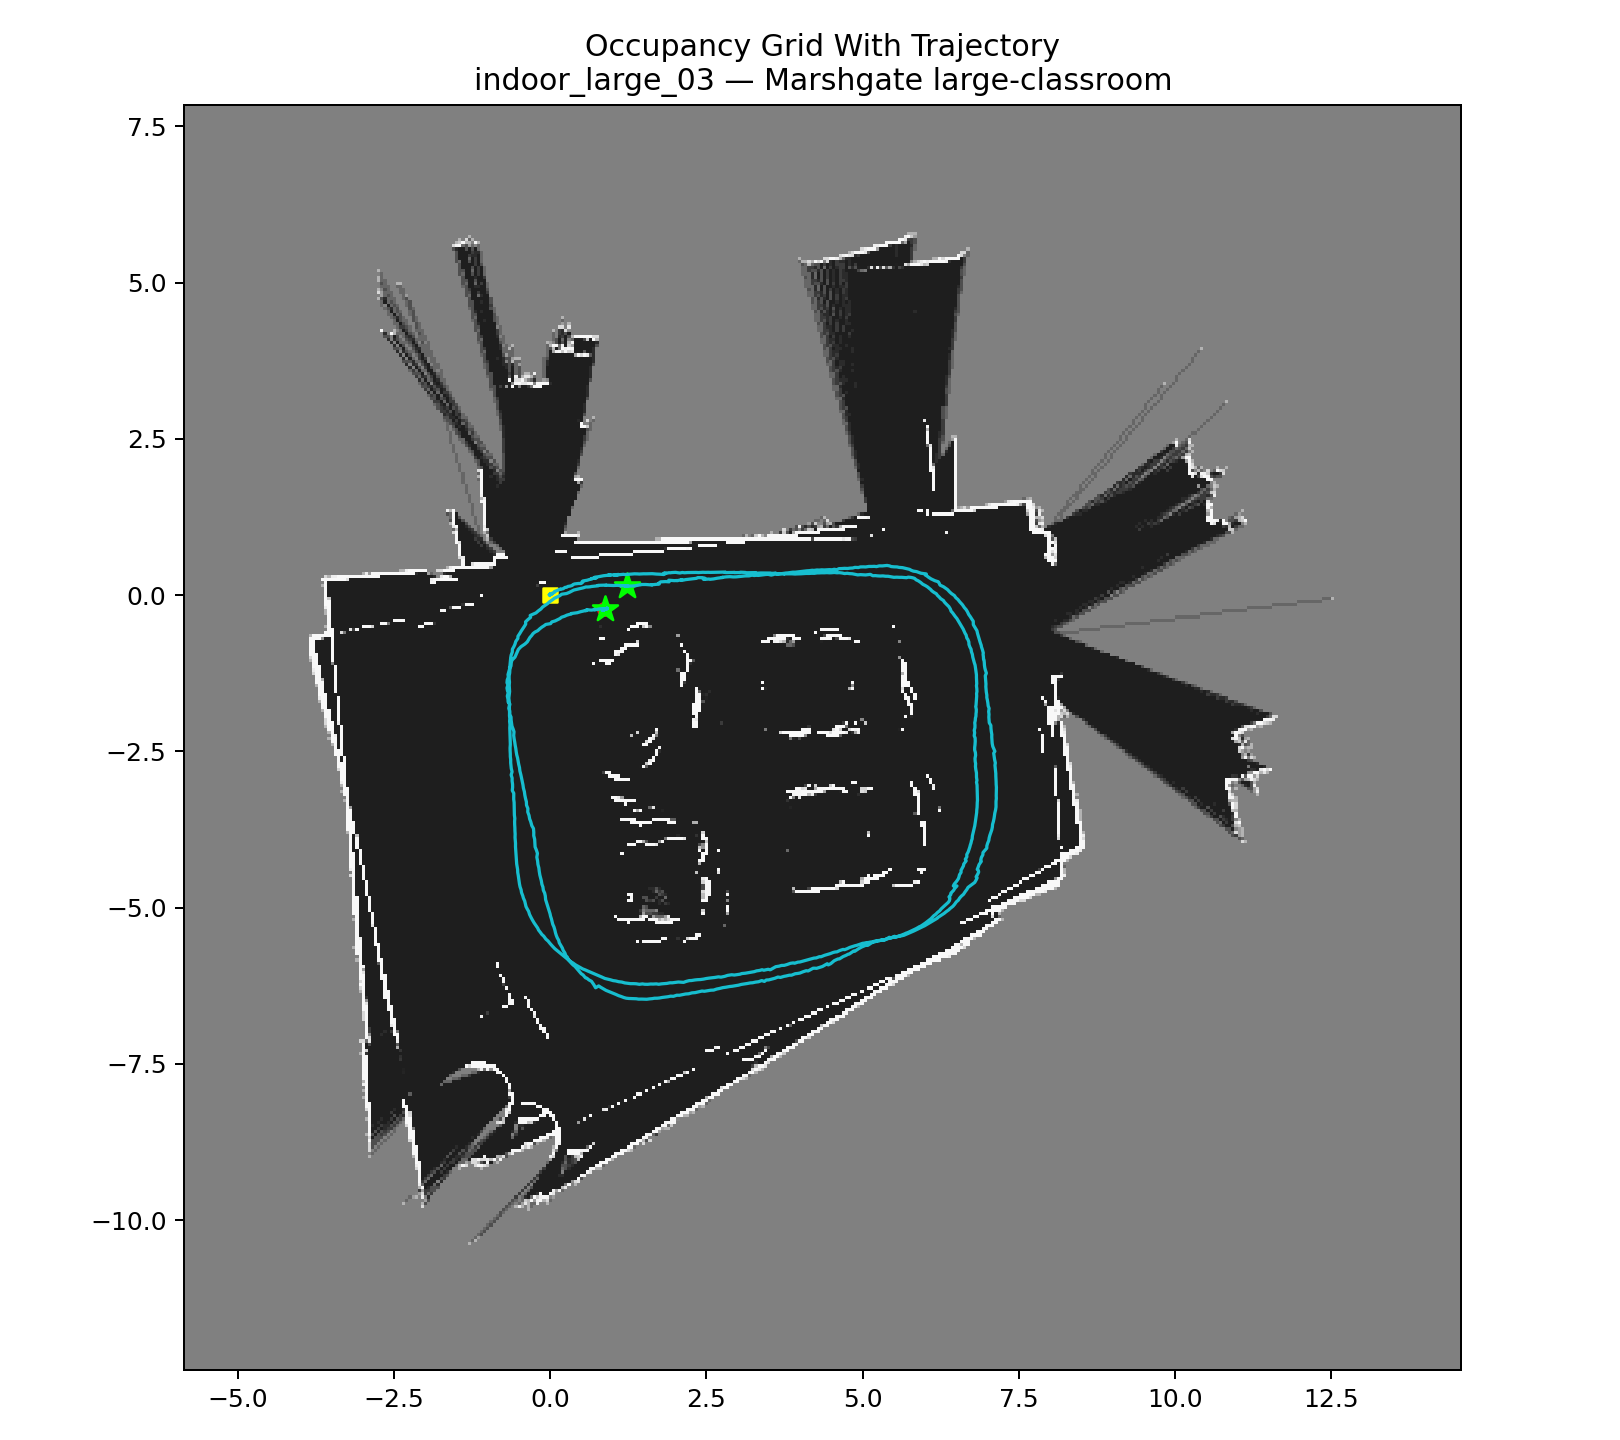
\includegraphics[width=\textwidth]{baseline_indoor_large.png}
      \centering\scriptsize Large classroom
    \end{column}
    \begin{column}{0.32\textwidth}
      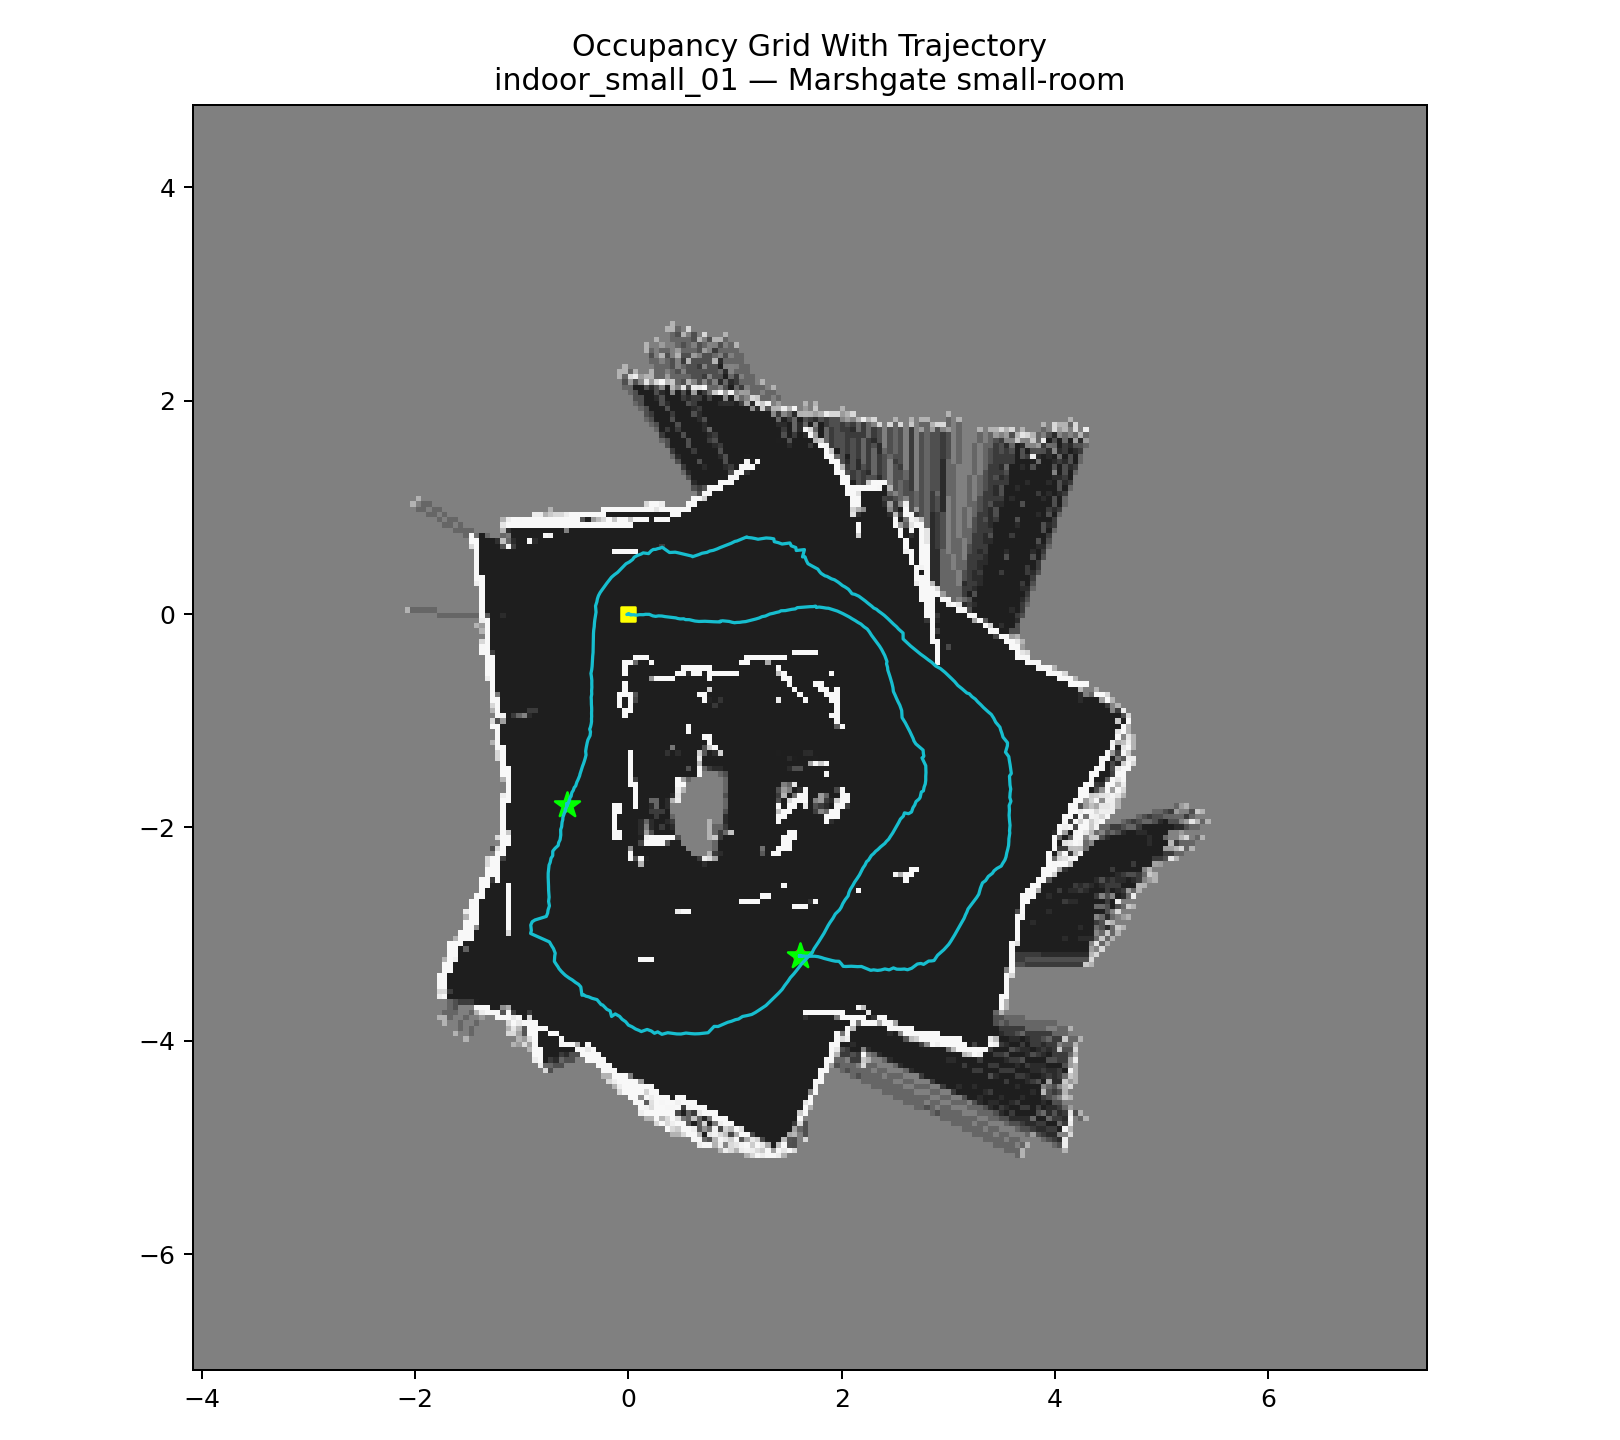
\includegraphics[width=\textwidth]{baseline_indoor_small.png}
      \centering\scriptsize Small room
    \end{column}
    \begin{column}{0.32\textwidth}
      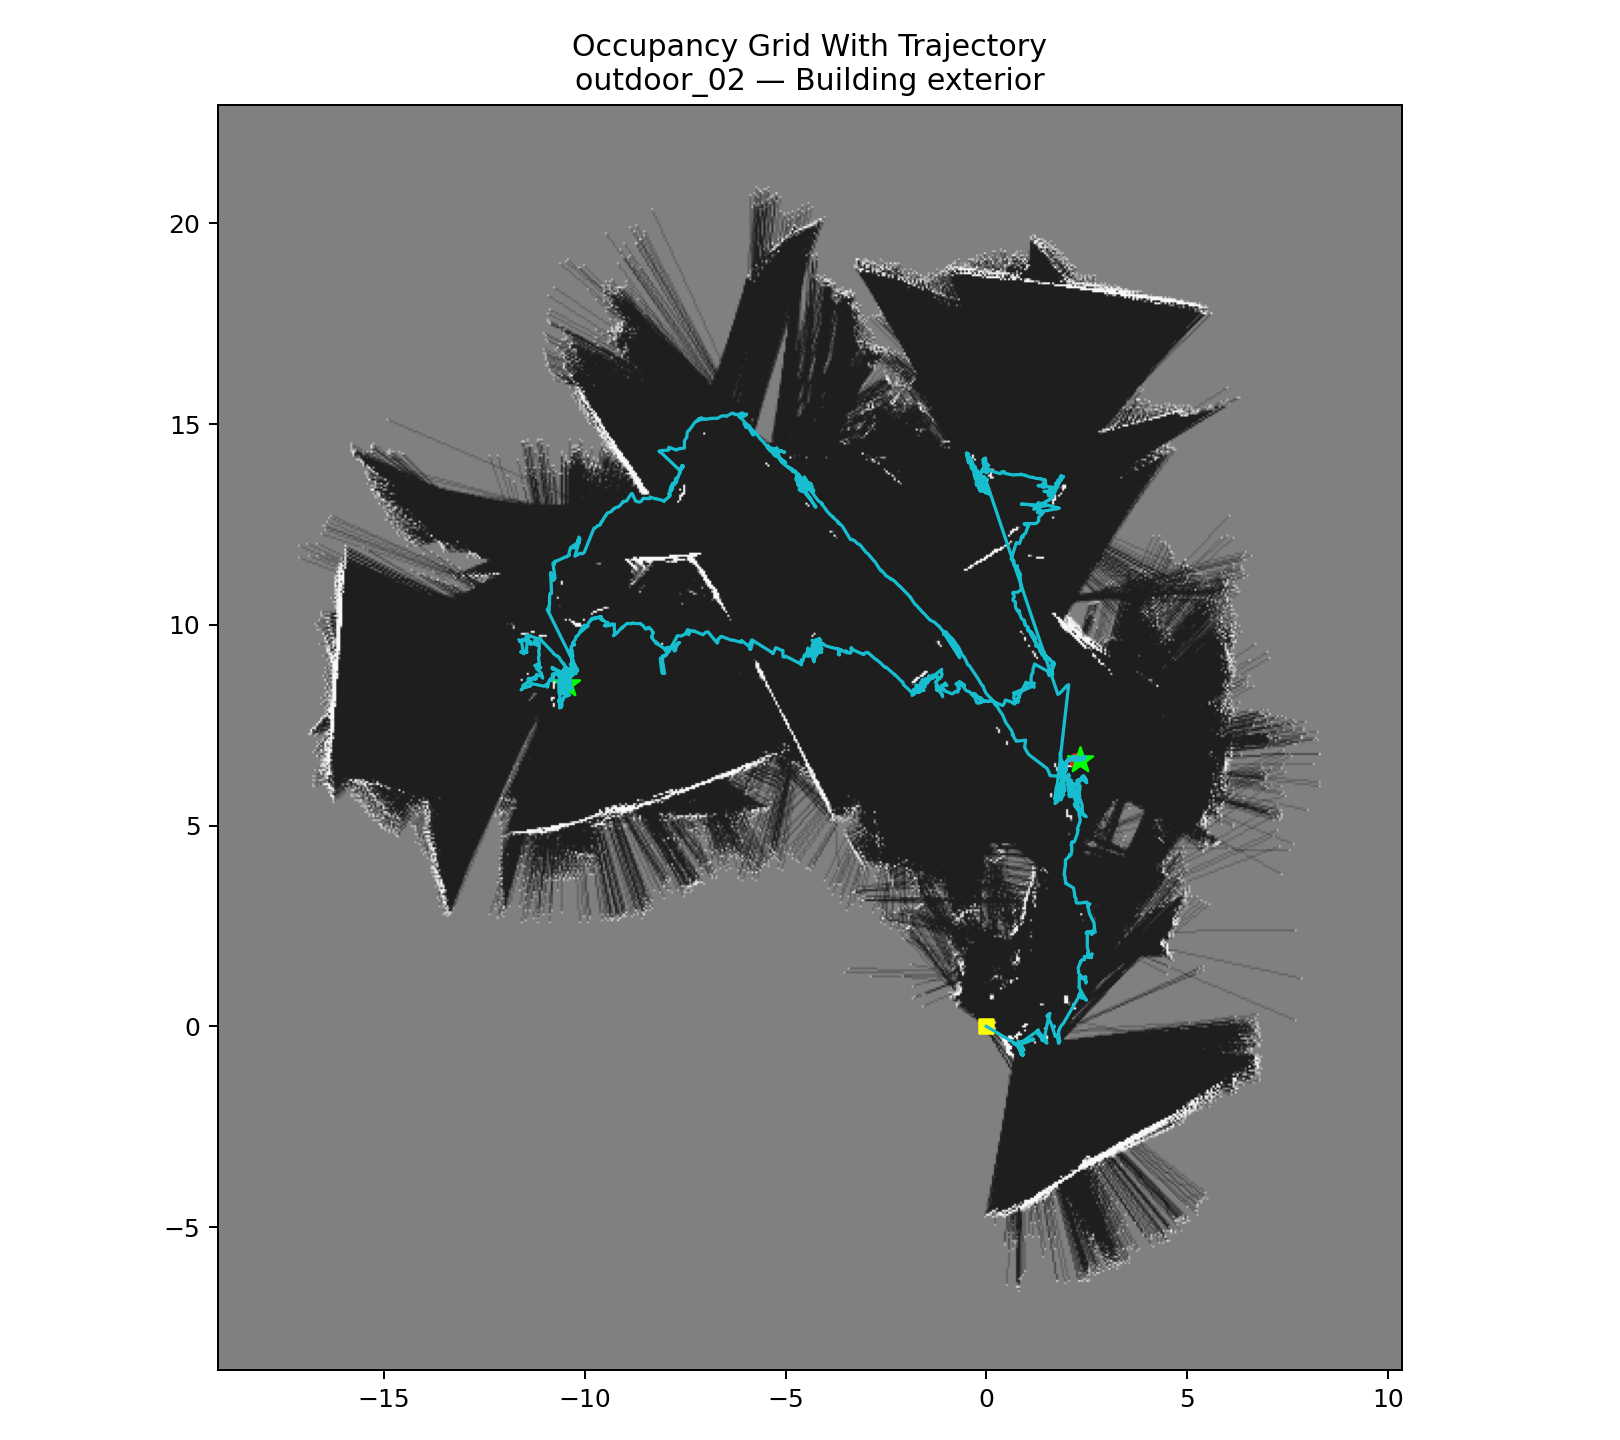
\includegraphics[width=\textwidth]{baseline_outdoor.png}
      \centering\scriptsize Outdoor
    \end{column}
  \end{columns}
\end{frame}

\end{document}
